\chapter{Export und Import}
\label{ch:exportImport}
\textit{Nicht nur in der Wirtschaft spielen Import und Export eine wichtige Rolle. Auch PUMA ist global vernetzbar.}
\section{Literaturlisten exportieren}
\label{sec:llExportieren}
PUMA ermöglicht den vollständigen Export\index{Export} von Publikationslisten aus PUMA in andere Programme. Das gängigste Datenformat, dass die meisten Programme unterstützen, ist BibTex\index{BibTex}. \newline 
Der Export erfolgt in zwei Schritten. Es wird zuerst ein Literaturverzeichnis in Puma zusammengestellt und exportiert, bevor es dann in das andere Programm importiert wird.
\subsection{Literaturverzeichnis zusammenstellen}
\label{subsec:lvZusammenstellen}
\begin{enumerate}
    \item Um ein Literaturverzeichnis zusammenzustellen, müssen Sie im ersten Schritt die Publikationen, die in Ihrem Verzeichnis abgelegt werden sollen, in Ihre Ablage\index{Ablage} kopieren. Hierfür gehen Sie in Ihre persönliche Publikations- und Lesezeichensammlung über den @Ihr Benutzername-Button oder klicken im Dropdown-Menü von \enquote{meinPUMA} auf \enquote{meine Einträge}.  Neben jeder Publikation befindet sich eine Symbolleiste.
    \item Klicken Sie auf das Aktenordner-Symbol (\enquote{Diese Publikation zur Ablage hinzufügen}). Die Publikation gelangt nun automatisch in Ihre Ablage und wird dort gespeichert.
\begin{figure}[h!]
 \centering
 \fbox{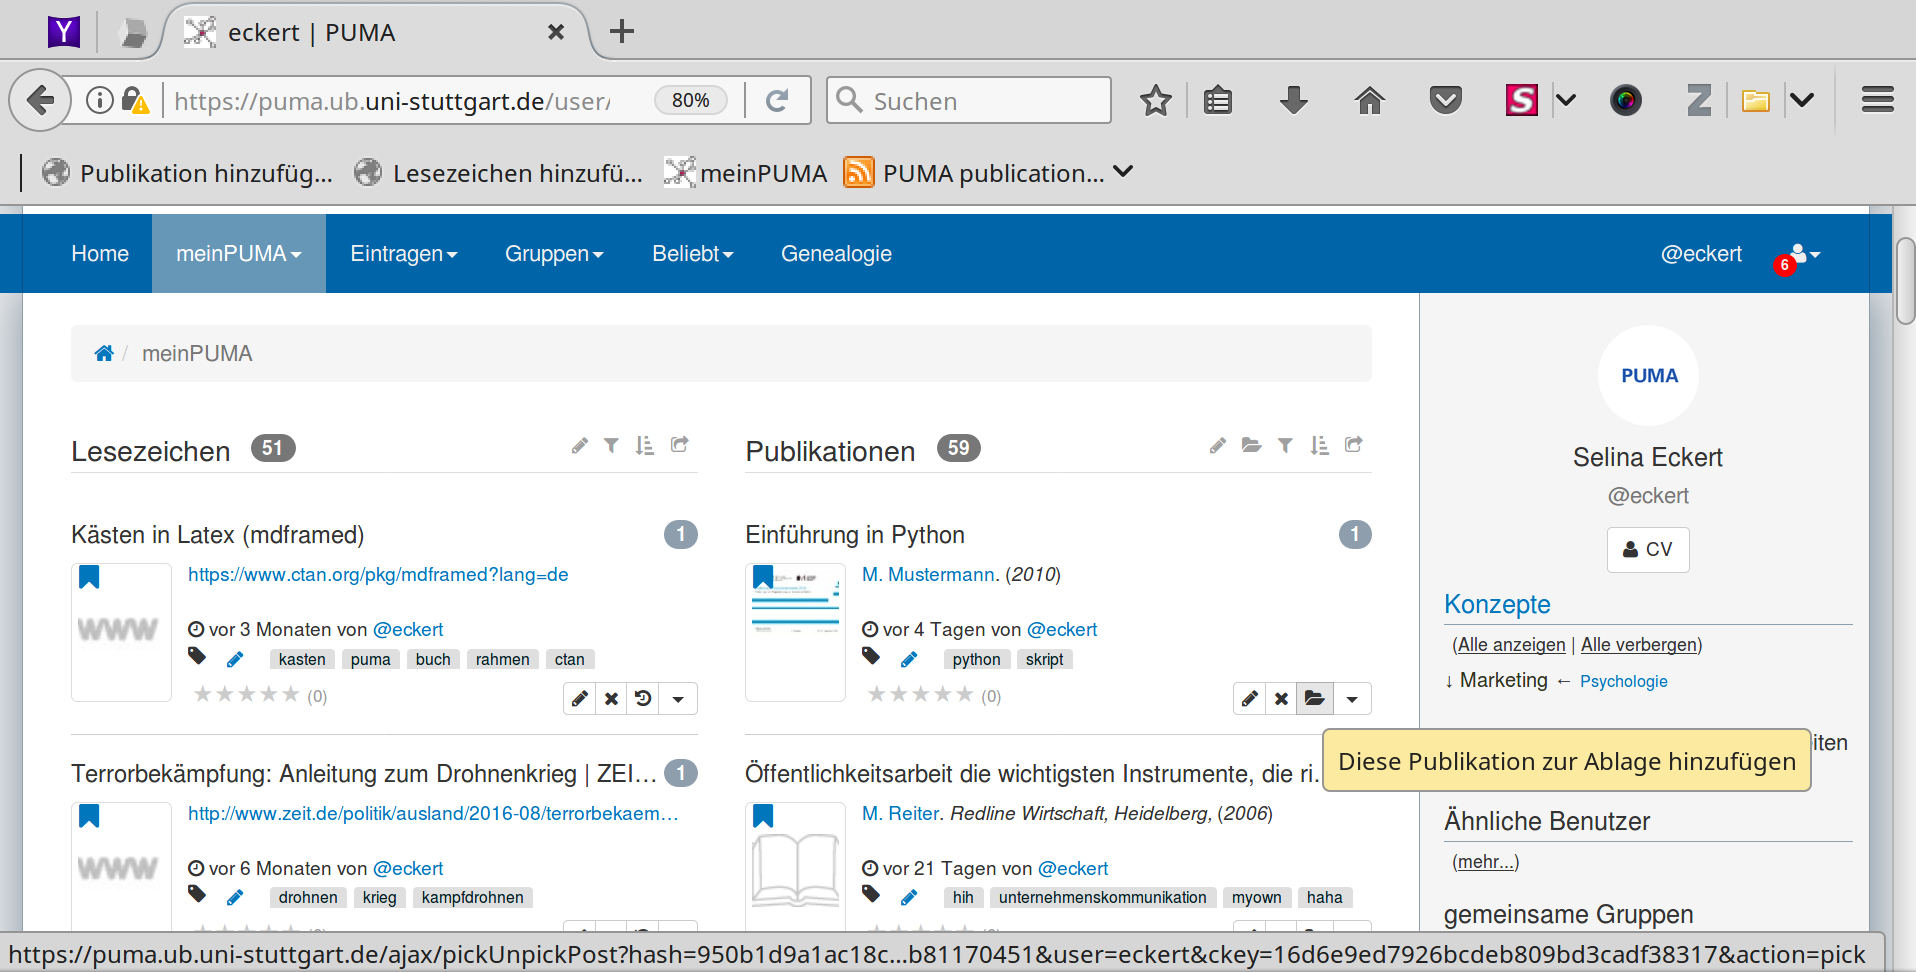
\includegraphics[width=10cm]{Bilder/Kapitel7/Zur_Ablage_hinzufuegen}}
 \caption{Zur Ablage hinzufügen}
 \label{fig:zurAblageHinzu}
\end{figure}
    \item Zur Ablage gelangen Sie über das Personensymbol. Klicken Sie im Dropdown-Menü auf \enquote{Ablage} und Ihnen werden alle Publikationen, die sich in Ihrer Ablage befinden angezeigt. 
\end{enumerate} 
Schnellerer Weg: Klicken Sie auf das Einstellungs-Zahnrad im Inhaltsbereich über den Publikationen. Wählen Sie unter der Rubrik \enquote{Ablage} \enquote{alle hinzufügen} aus. Alle Publikationen aus dem Inhaltsbereich werden in die Ablage übernommen. 
\subsection{Literaturverzeichnis exportieren}
\label{subsec:lvExportieren}
\textbf{Voraussetzung:} Sie haben ein Literaturverzeichnis zusammengestellt.
\begin{enumerate}
    \item Klicken Sie in der Ablage auf das Exportzeichen oben rechts. Ein Dropdown-Menü erscheint.
\begin{figure}[h!]
 \centering
 \fbox{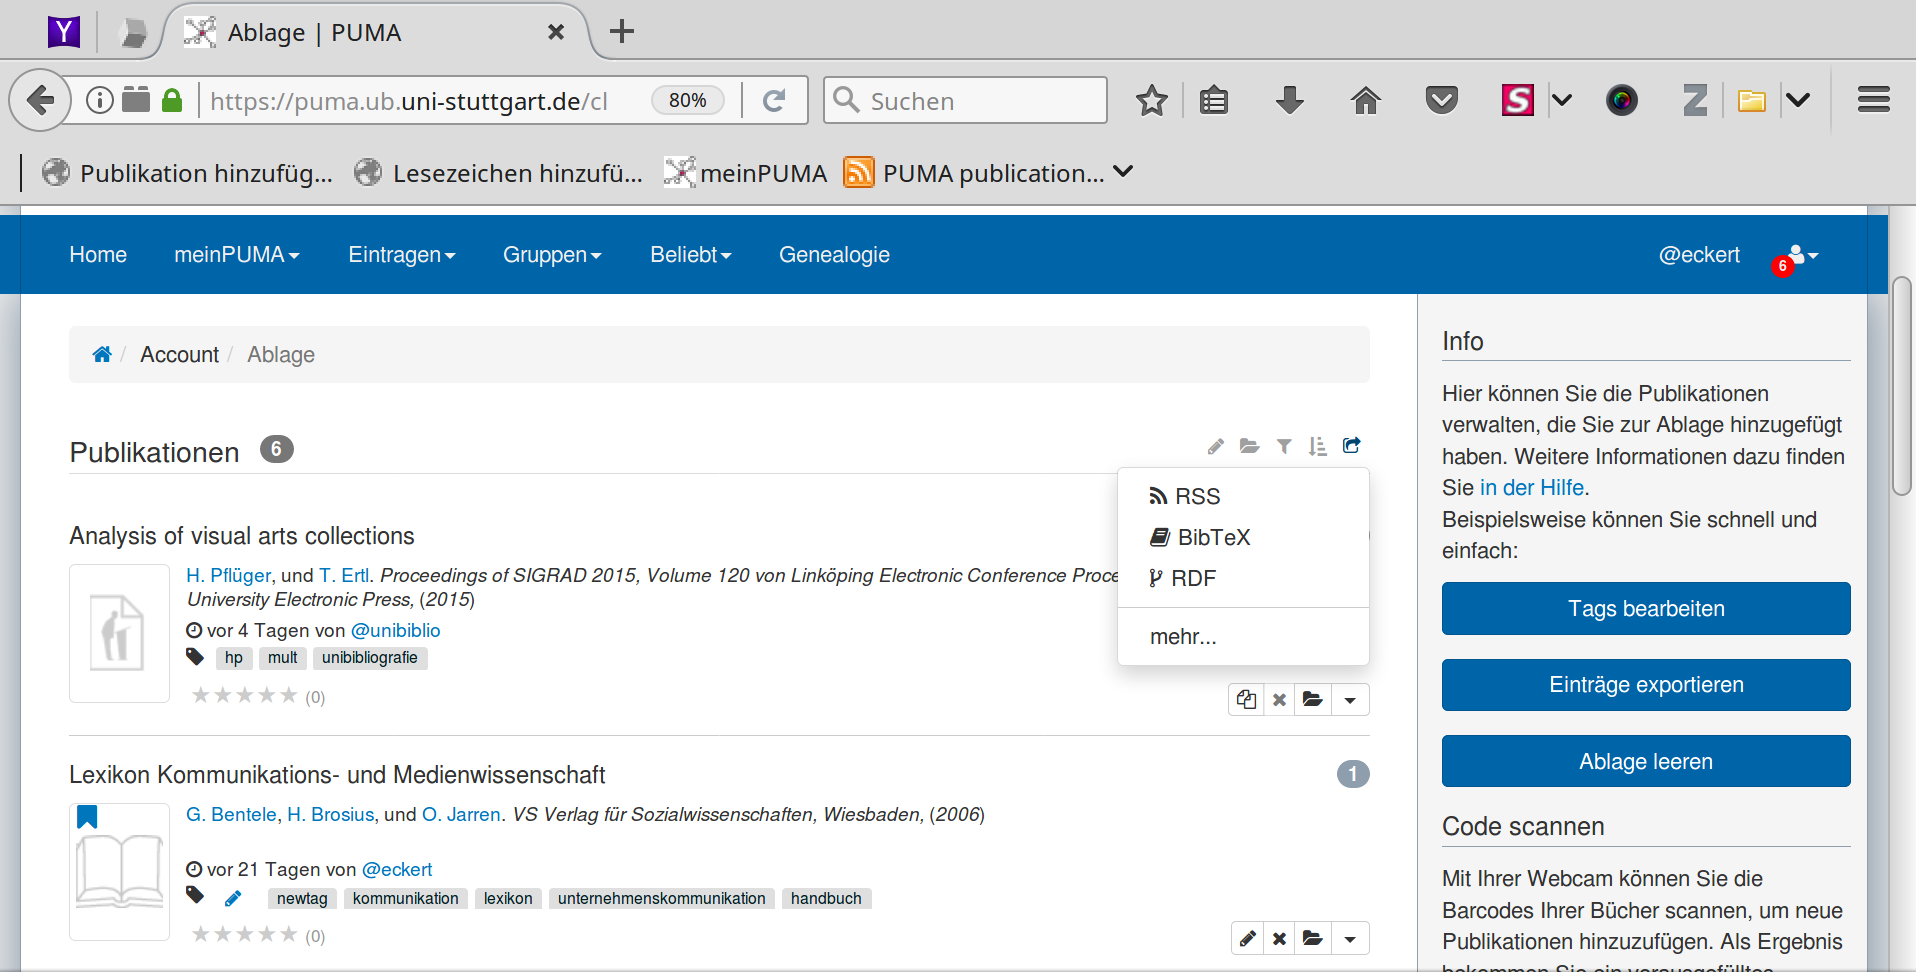
\includegraphics[width=11cm]{Bilder/Kapitel7/Exportformat_auswaehlen}}
 \caption{Das Exportformat auswählen}
 \label{fig:exportformatAuswaehlen}
\end{figure}
    \item Wählen Sie das Format, in dem Sie ihr Literaturverzeichnis haben möchten. PUMA gibt Ihnen einige Beispiele vor (RSS, BibTex, RDF). Klicken Sie auf \enquote{mehr...} haben Sie auch die Möglichkeit Ihr Literaturverzeichnis mit weiteren Formaten zu exportieren. 
\begin{figure}[h!]
 \centering
 \fbox{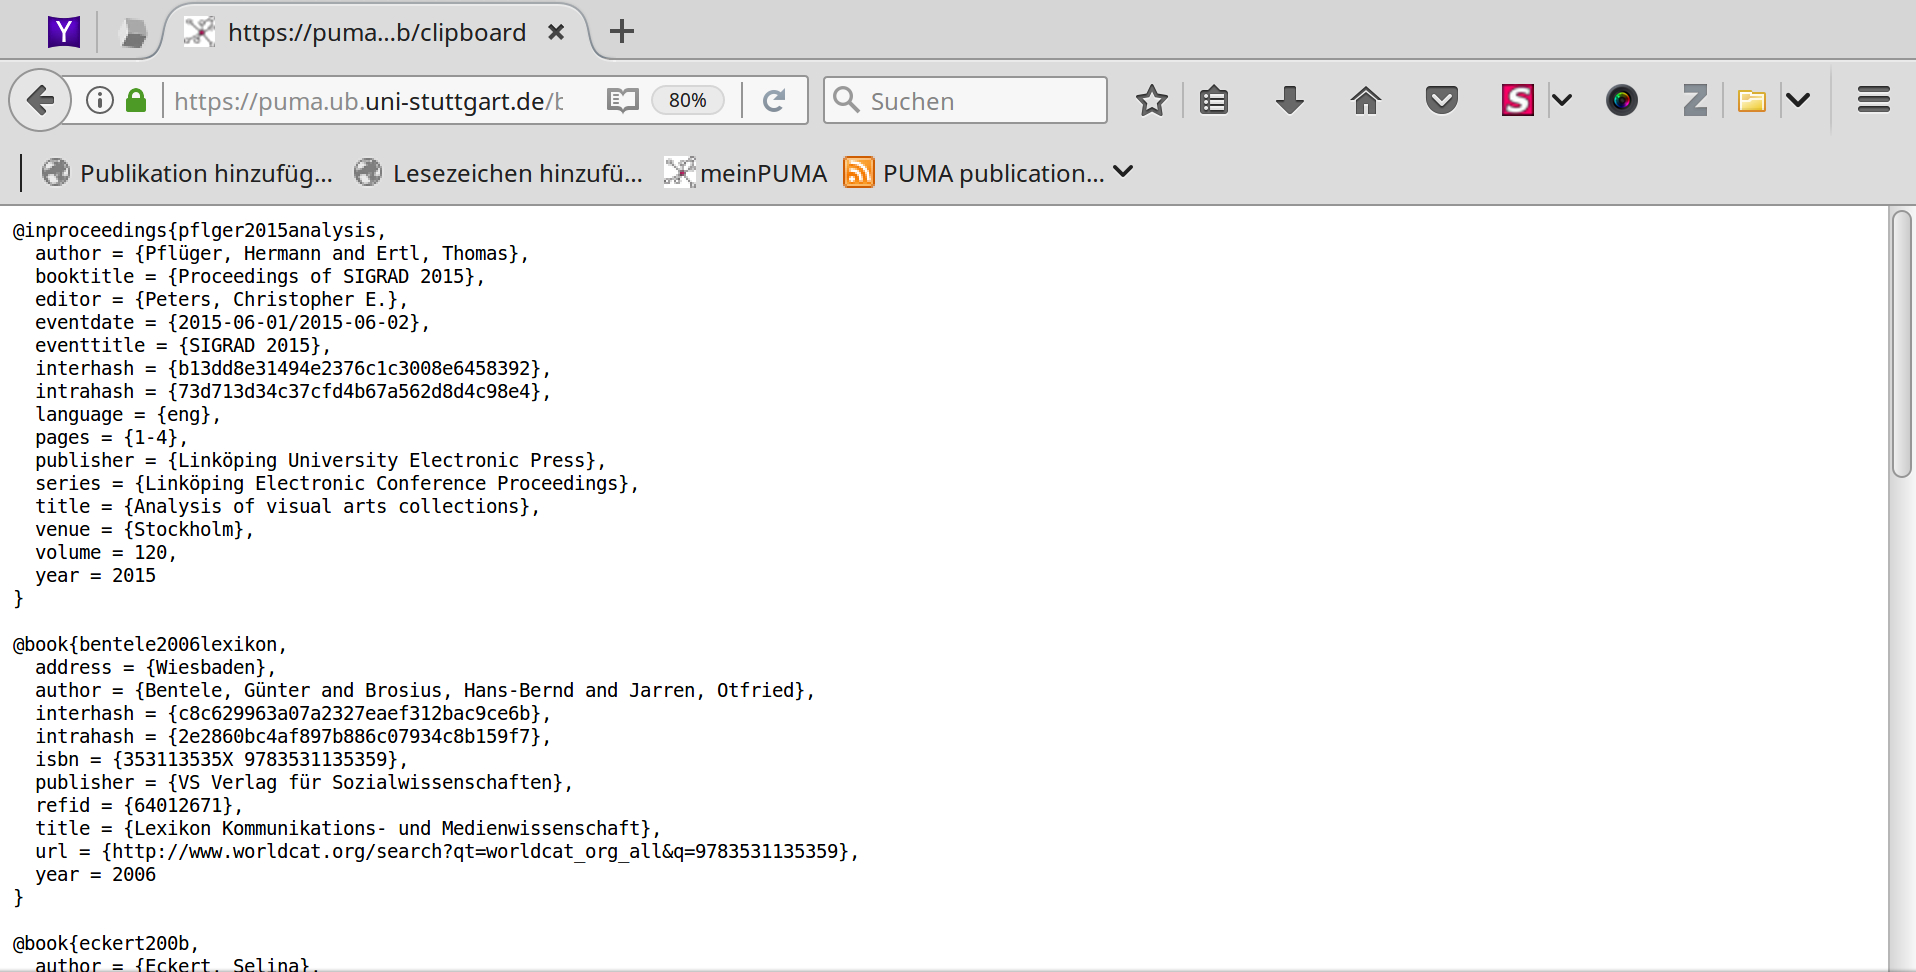
\includegraphics[width=11cm]{Bilder/Kapitel7/Das_Literaturverzeichnis}}
 \caption{Das Literaturverzeichnis}
 \label{fig:literaturverzeichnis}
\end{figure}
\begin{mdframed}[style=mdfexample1,frametitle={\texttt{TIPP}},backgroundcolor=gray!40] \texttt{Der Gebrauch des BibTex-Formates\index{BibTex} ist zu empfehlen, da dieses Format sehr verbreitet ist.}
\end{mdframed}
    \item Sobald Sie das gewählte Format angeklickt haben erscheint ein neues Fenster. Klicken Sie mit der rechten Maustaste auf die Seite und wählen \enquote{Speichern unter} um die Datei zu speichern.
\end{enumerate}
\subsection{Literaturverzeichnis exportieren- Programmspezifisch}
\label{subsec:lvExportProgramme}
\subsubsection*{Export nach Word\index{Export!Word}} \index{Word} \label{sss:exportWord}
\begin{enumerate}
    \item Klicken Sie in der Ablage auf das Exportzeichen.
    \item Wählen Sie im Dropdown-Menü \enquote{mehr...} aus.
    \item Es öffnet sich die Übersichtsseite der Exportformate. Wählen Sie das Format \enquote{MSOffice XML\index{MSOffice XML}}. Speichern Sie anschließend die Datei.
\begin{figure}[h!]
 \centering
 \fbox{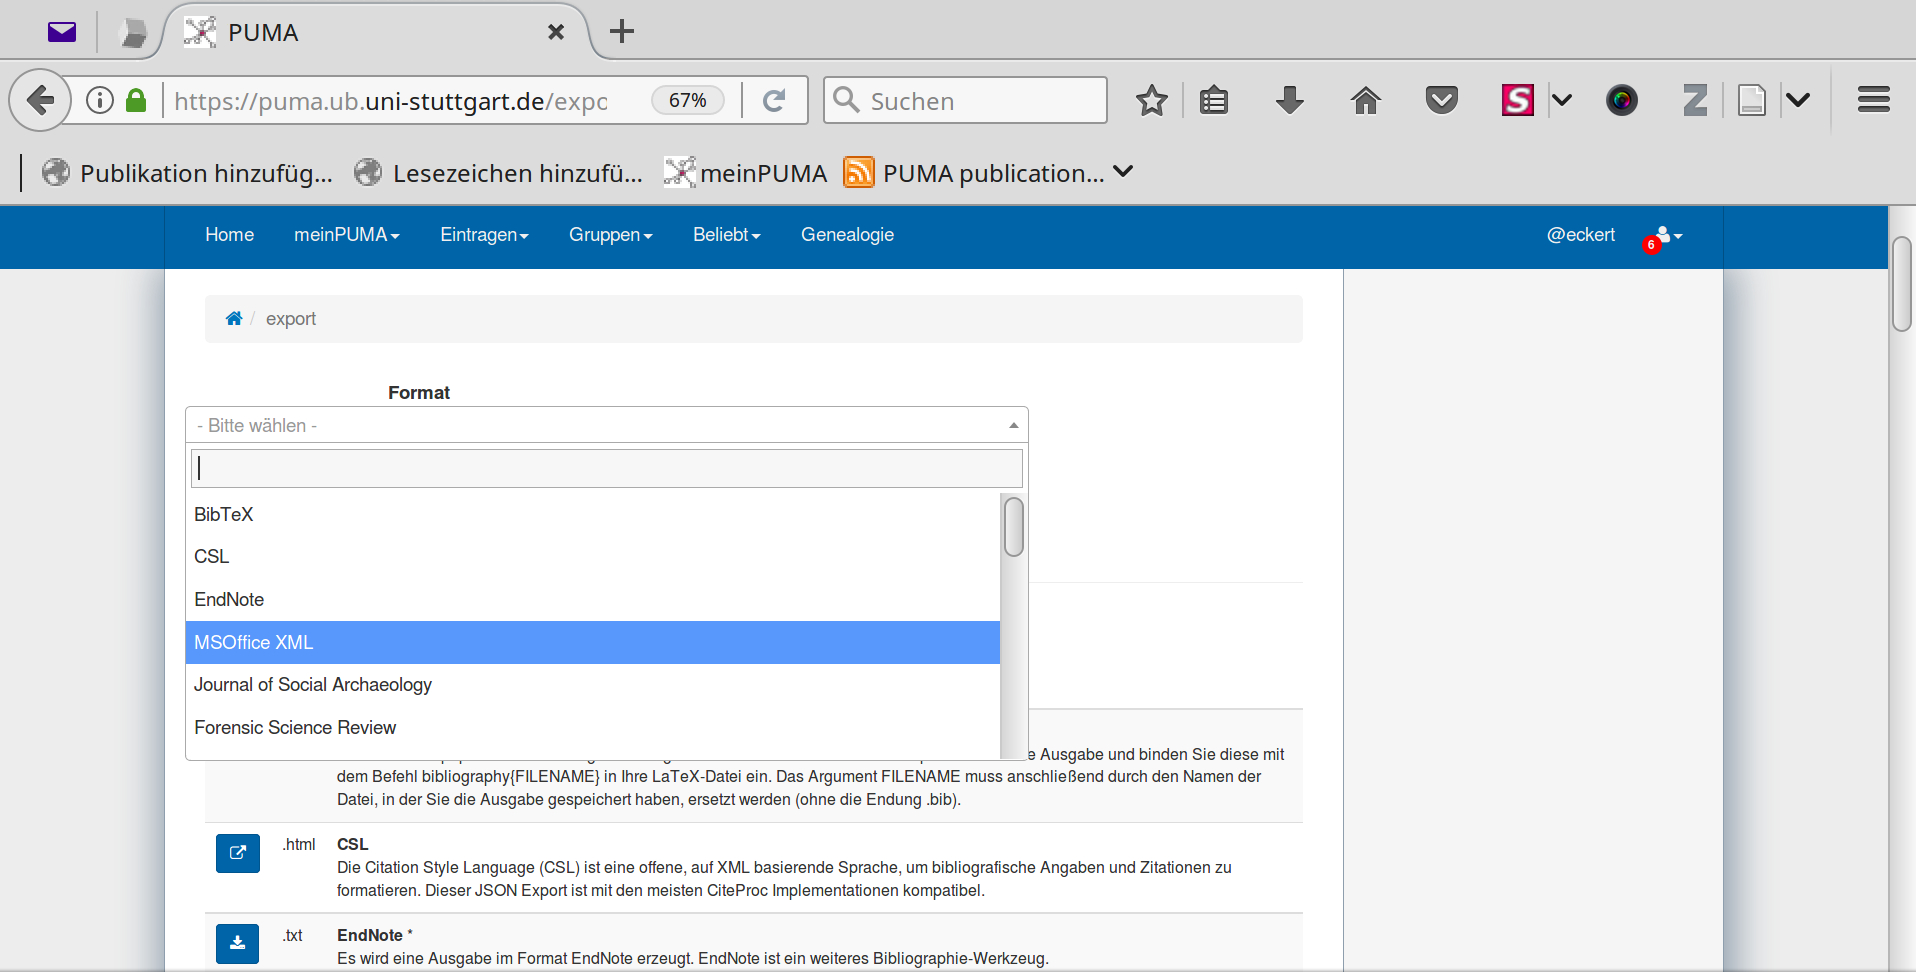
\includegraphics[width=11cm]{Bilder/Kapitel7/MSOffice_XML}}
 \caption{Das Exportformat MSOffice XML}
 \label{fig:exportformatMSOfficeXml}
\end{figure}
    \item In Microsoft Word können Sie nun die gespeicherte Datei hochladen, indem Sie unter \enquote{Verweise} auf \enquote{Quellen verwalten} klicken. Im erscheinenden Dialog (Quellen-Manager) können Sie auf \enquote{Durchsuchen} klicken und die gespeicherte Datei auswählen.
\begin{figure}[h!]
 \centering
 \fbox{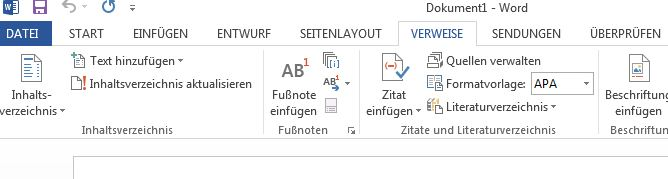
\includegraphics[width=11cm]{Bilder/Kapitel7/Word}}
 \caption{Reiter Verweise}
 \label{fig:reiterVerweise}
\end{figure}
\begin{figure}[h!]
 \centering
 \fbox{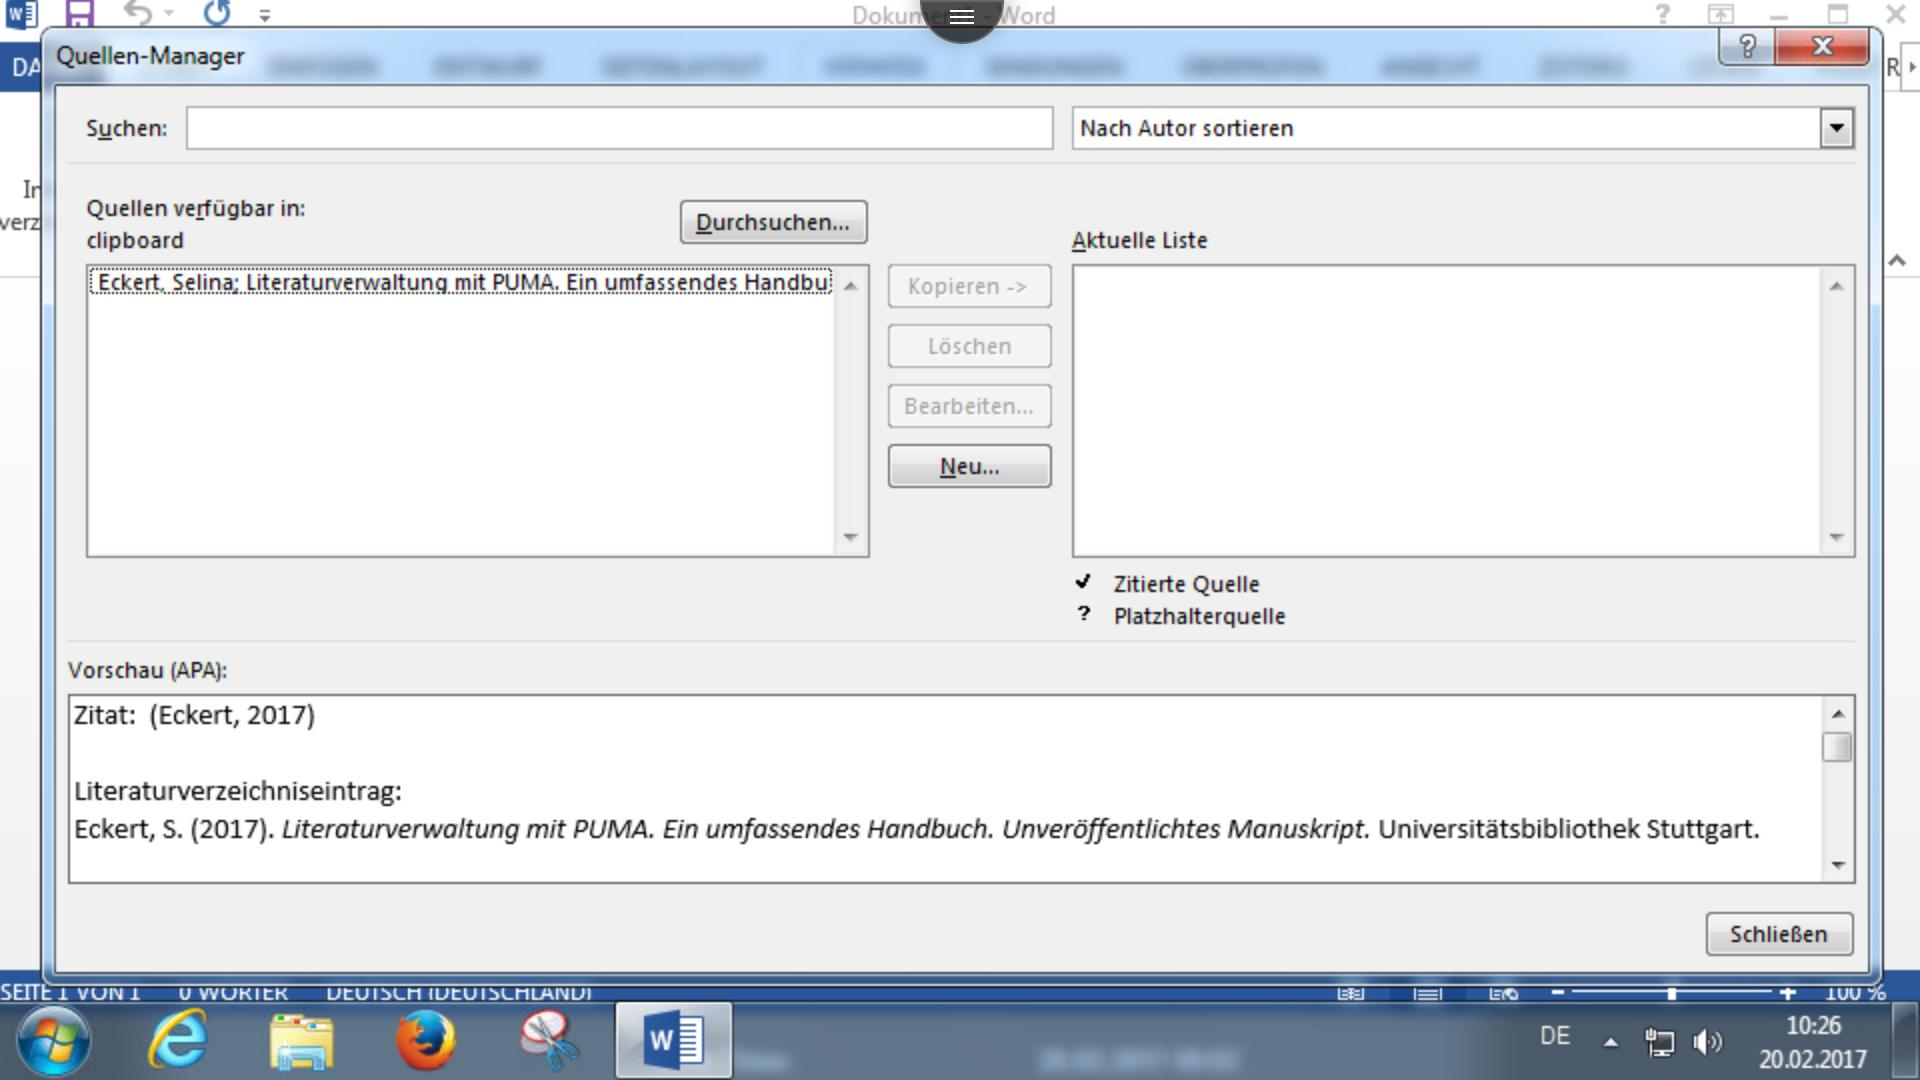
\includegraphics[width=11cm]{Bilder/Kapitel7/Quellen-Manager}}
 \caption{Quellen-Manager}
 \label{fig:quellenManager}
\end{figure} 
    \item Kopieren Sie Quellen in die aktuelle Liste, durch markieren der entsprechenden Quellen und klicken auf \enquote{Kopieren}. Schließen Sie anschließend das Fenster.
    \item Sie können sich nun das Literaturverzeichnis anzeigen lassen, indem Sie auf \enquote{Literaturverzeichnis} klicken und sich das gewünschte Layout aussuchen.
\end{enumerate}
\subsubsection*{Export nach Citavi\index{Export!Citavi}}\label{sss:exportCitavi}
\begin{enumerate}
	\item Klicken Sie auf den Titel der Publikation, die Sie nach Citavi\index{Citavi} importieren möchten.
	\item Es öffnet sich die Detailansicht der Publikation. Wählen Sie unten auf der Seite unter \enquote{Zitieren Sie diese Publikation} den Stil \enquote{BibTex\index{BibTex}} aus. 
	\item Markieren Sie die Zitation im Textfeld und kopieren Sie diese in die Zwischenablage. Benutzen Sie hierfür entweder STRG+C oder über die rechte Maustaste und \enquote{Kopieren}.
	\item Öffnen Sie Citavi. Klicken Sie in der Menüleiste oben links auf \enquote{Datei}.
	\item Wählen Sie im Dropdown-Menü \enquote{Importieren} aus. Es öffnet sich ein Popup-Fenster.
	\item Wählen Sie \enquote{Aus einer Textdatei (Ris-, BibTex-formatiert o.ä.)} aus. Klicken Sie anschließend auf \enquote{Weiter}.
	\item Wählen Sie auf der nächsten Seite BibTex als Format aus. Anschließend klicken Sie auf \enquote{Weiter}.
	\item Wählen Sie \enquote{Textdaten in der Zwischenablage verwenden} aus und klicken anschließend auf \enquote{Weiter}.
	\item Setzen Sie ein Häkchen bei \enquote{Importierte BibTex Keys ersetzen}. Klicken Sie auf \enquote{Weiter}.
	\item Wählen Sie im letzten Schritt die entsprechende Datei aus und klicken auf \enquote{Titel übernehmen}. Sie werden gefragt, ob Sie die Tags mit übernehmen möchten, setzen Sie für die Übernahmen ein Häkchen und klicken auf \enquote{OK}.
\end{enumerate}




\subsubsection*{Export nach Zotero\index{Export!Zotero}}\label{sss:exportZotero}
\begin{enumerate}
    \item Sie befinden sich auf einer PUMA-Seite (z.B. die Home-Seite oder Ihre Benutzerseite), von der Sie eine Publikation in Ihre Zotero-Bibliothek übernehmen möchten. Klicken Sie auf den schwarzen Pfeil neben dem Zotero\index{Zotero}-Symbol oben rechts bei Firefox.
    \item Ein Dropdown-Menü öffnet sich. Wählen Sie \enquote{In Zotero mit \enquote{unAPI} speichern}.
    
\begin{figure}[h!]
 \centering
 \fbox{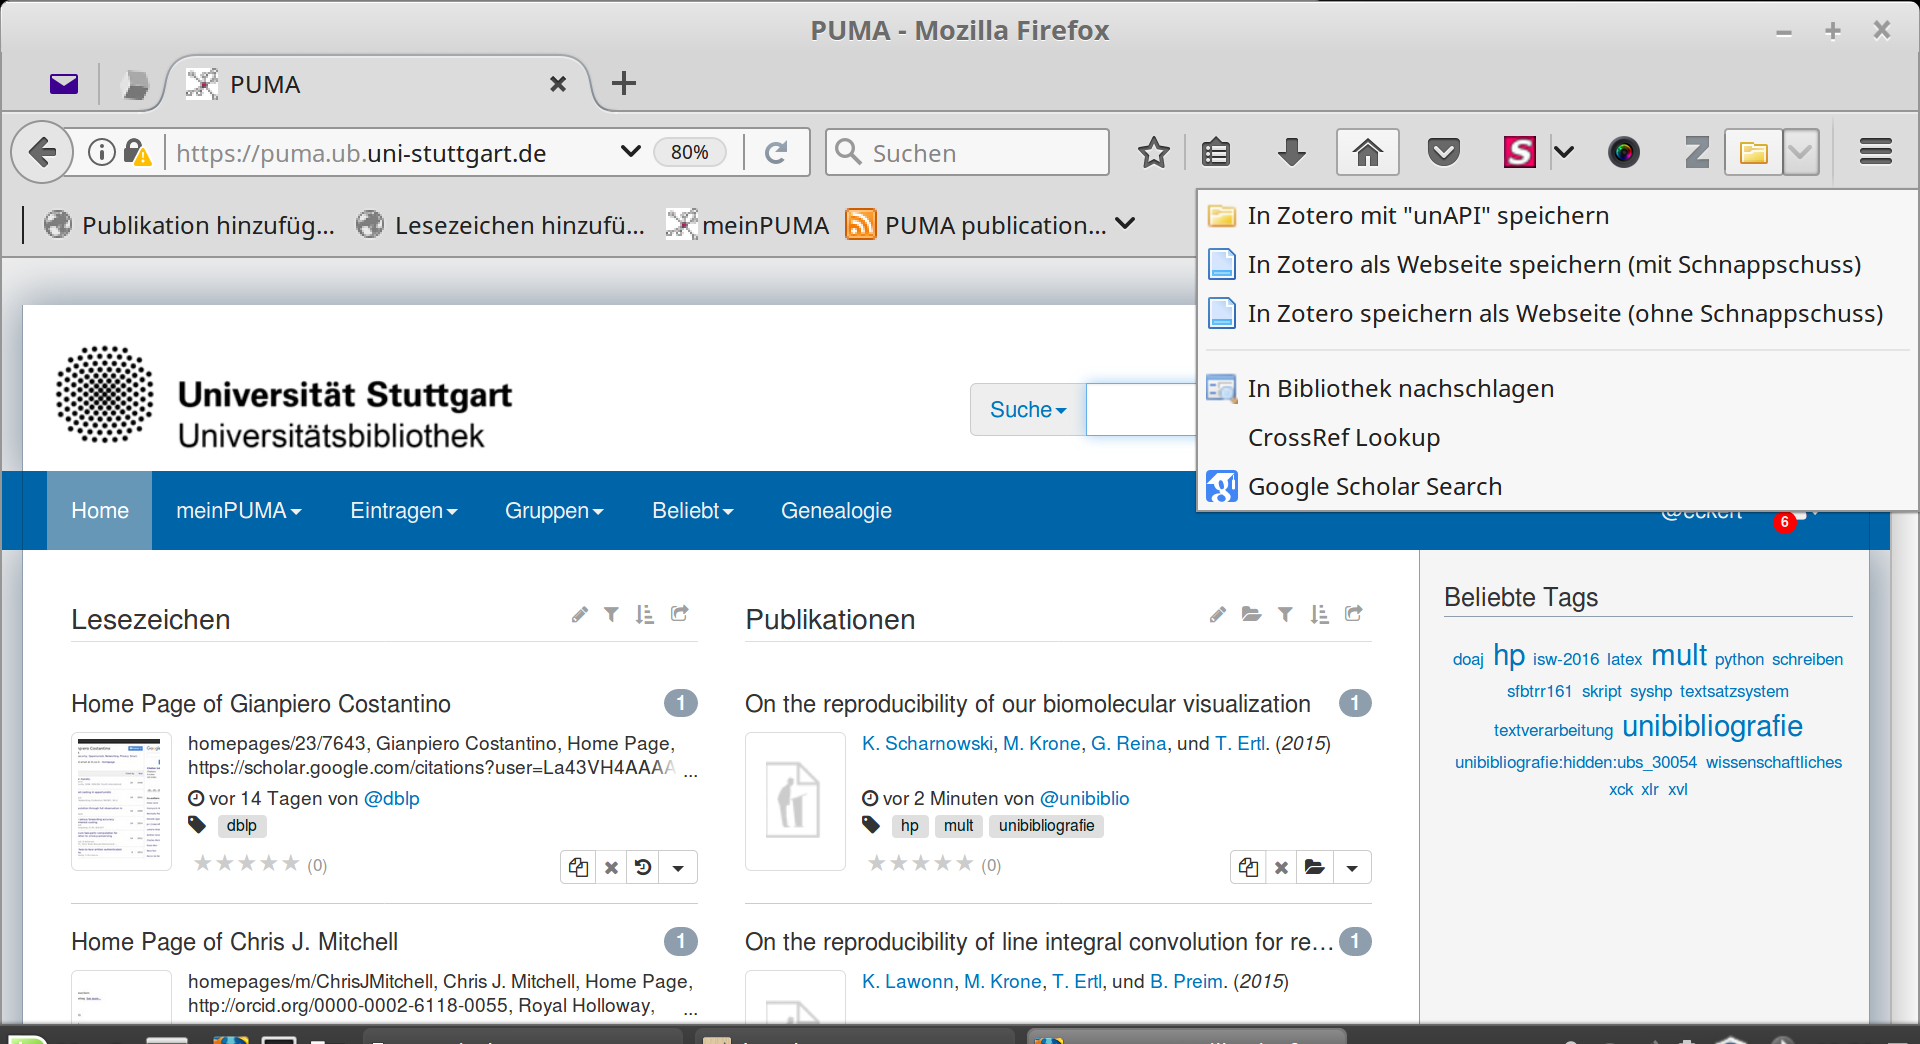
\includegraphics[width=10cm]{Bilder/Kapitel7/Zotero_Dropdown_Menue}}
 \caption{Dropdown-Menü}
 \label{fig:dropdownMenue}
\end{figure}

    \item Es öffnet sich ein Popup-Fenster, in dem alle Publikationen der entsprechenden PUMA-Seite aufgelistet sind. Wählen Sie die Publikationen aus, die Sie in Ihre Zotero-Bibliothek übernehmen möchten. Bestätigen Sie anschließend Ihre Wahl mit \enquote{OK} und Ihre ausgewählten Einträge erscheinen in Ihrer Zotero-Bibliothek.

\begin{figure}[h!]
 \centering
 \fbox{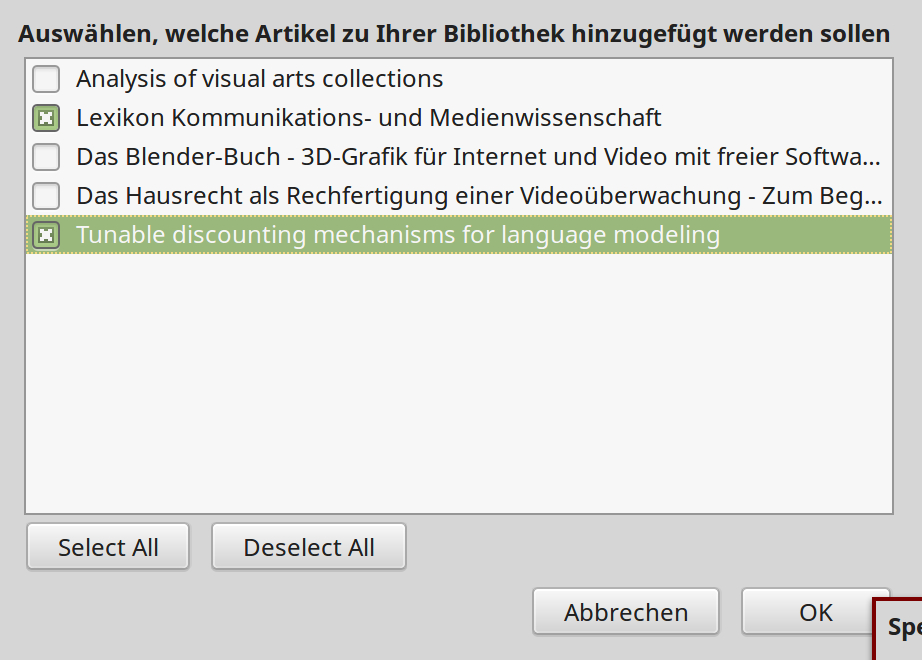
\includegraphics[width=10cm]{Bilder/Kapitel7/Zotero_Eintraege_auswaehlen}}
 \caption{Einträge auswählen}
 \label{fig:eintraegeAuswaehlen}
\end{figure}

\end{enumerate} 
\subsubsection*{Export nach JabRef\index{Export!JabRef}}\label{sss:exportJabref}
\begin{enumerate}
    \item Legen Sie alle Publikationen, die Sie in JabRef\index{JabRef} exportieren möchten in Ihre Anlage.
    \item Klicken Sie aus das Exportzeichen oben rechts in der Ablage und wählen Sie im Dropdown- Menü das Dateiformat \enquote{BibTex} aus.
    \item Ihre Publikationen werden Ihnen anschließend dem ausgewählten Dateiformat angezeigt. Drücken Sie auf die rechte Maustaste und speichern Sie die Publikationen, indem Sie \enquote{Speichern unter...} wählen, an dem gewünschten Platz. 
    \item Öffnen Sie JabRef und klicken auf den Reiter \enquote{Datei}. 
    \item Es öffnet sich ein Dropdown-Menü. Wählen Sie zwischen den Optionen: \enquote{Importieren in neue Datenbank} oder \enquote{Importieren in aktuelle Datenbank}.
    \item Auf dem Bildschirm erscheint ein Popup-Fenster, indem Sie, die in Schritt 3 abgespeicherte Datei, auswählen können. Bestätigen Sie anschließend Ihre Wahl mit \enquote{Öffnen}. Die Publikationen werden Ihnen in der ausgewählten Datenbank automatisch angezeigt.
\end{enumerate}

\section{Literaturlisten importieren}
\label{sec:llImportieren}
Das Importieren\index{Import} von Literaturlisten aus anderen Programmen in PUMA ist jederzeit möglich. Das gängigste Datenformat, das die meisten Programme unterstützen, ist BibTex\index{BibTex}. \newline 
Der Import erfolgt in zwei Schritten. Exportieren Sie zuerst die gewünschten Publikationen aus dem Litertaurverwaltungsprgramm, bevor Sie sie anschließend nach PUMA importieren. 
\subsection{BibTex-Export aus verwendeten Literaturverwaltungsprogrammen}
\label{subsec:bibtexExport}
\subsubsection*{Bib-TeX-Export aus Citavi\index{Import!Citavi}}\label{sss:importCitavi} 
\begin{enumerate}
    \item Klicken Sie bei Citavi\index{Citavi} oben rechts auf \enquote{Datei}, dann im Dropdown-Menü auf \enquote{Exportieren}.
    \item Ein Dialog erscheint. Wählen Sie aus, ob Sie nur den markierten oder alle Artikel exportieren möchten. Klicken Sie dann im Dialog unten auf \enquote{Weiter}.

\begin{figure}[h!]
 \centering
 \fbox{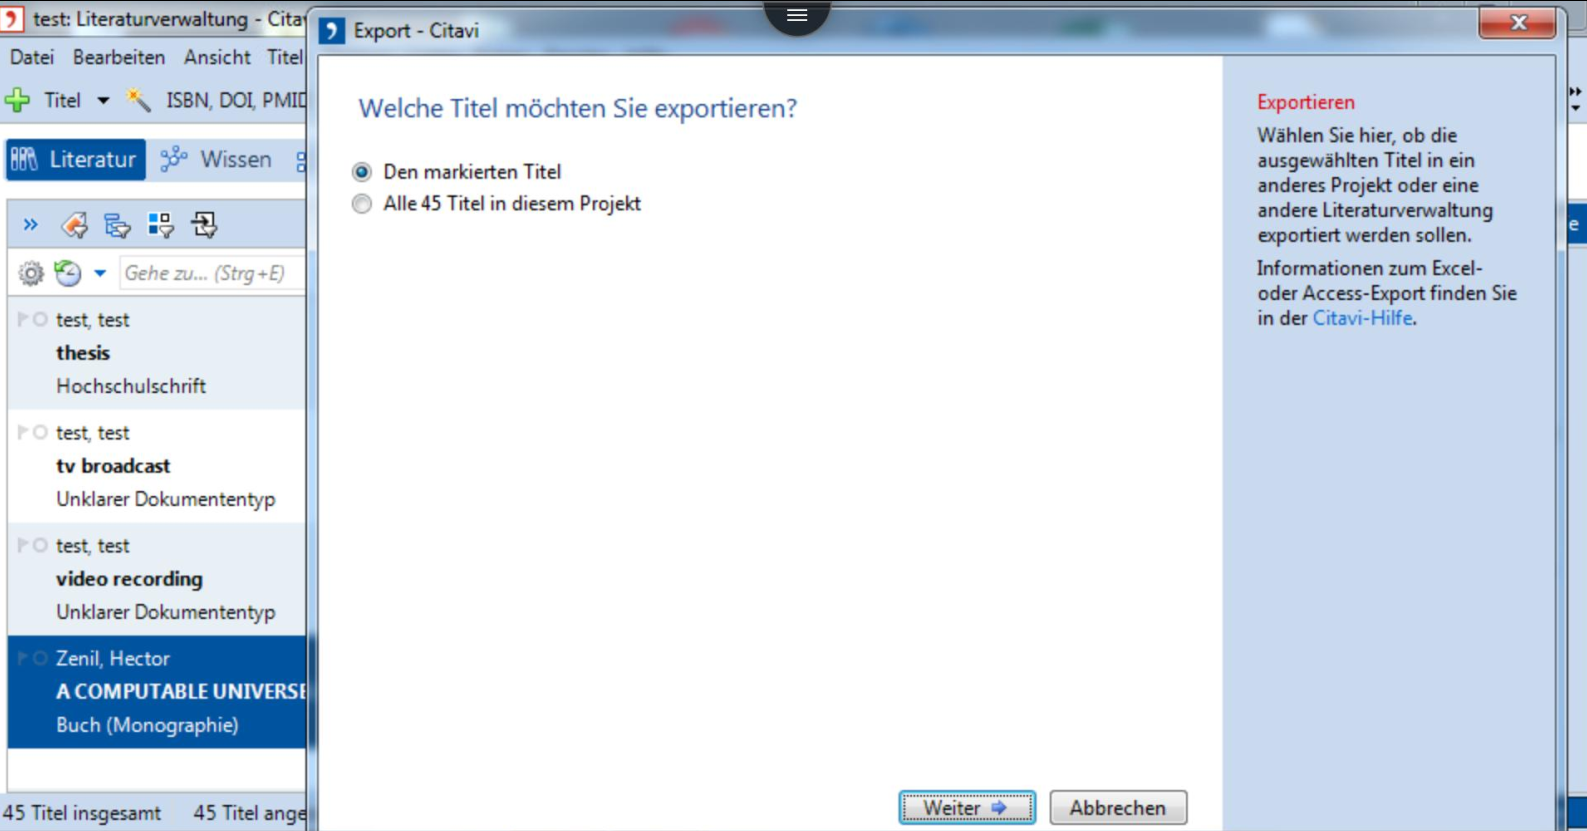
\includegraphics[width=9cm]{Bilder/Kapitel7/Citavi_Schritt2}}
 \caption{Auswählen der zu exportierenden Artikel}
 \label{fig:exportierendenArtikelAuswaehlen}
\end{figure}
    \item Im nächsten Schritt werden Sie nach dem Export-Format gefragt, wählen Sie hier \enquote{BibTex} aus und klicken anschließend auf \enquote{Weiter}.
  
\begin{figure}[h!]
 \centering
 \fbox{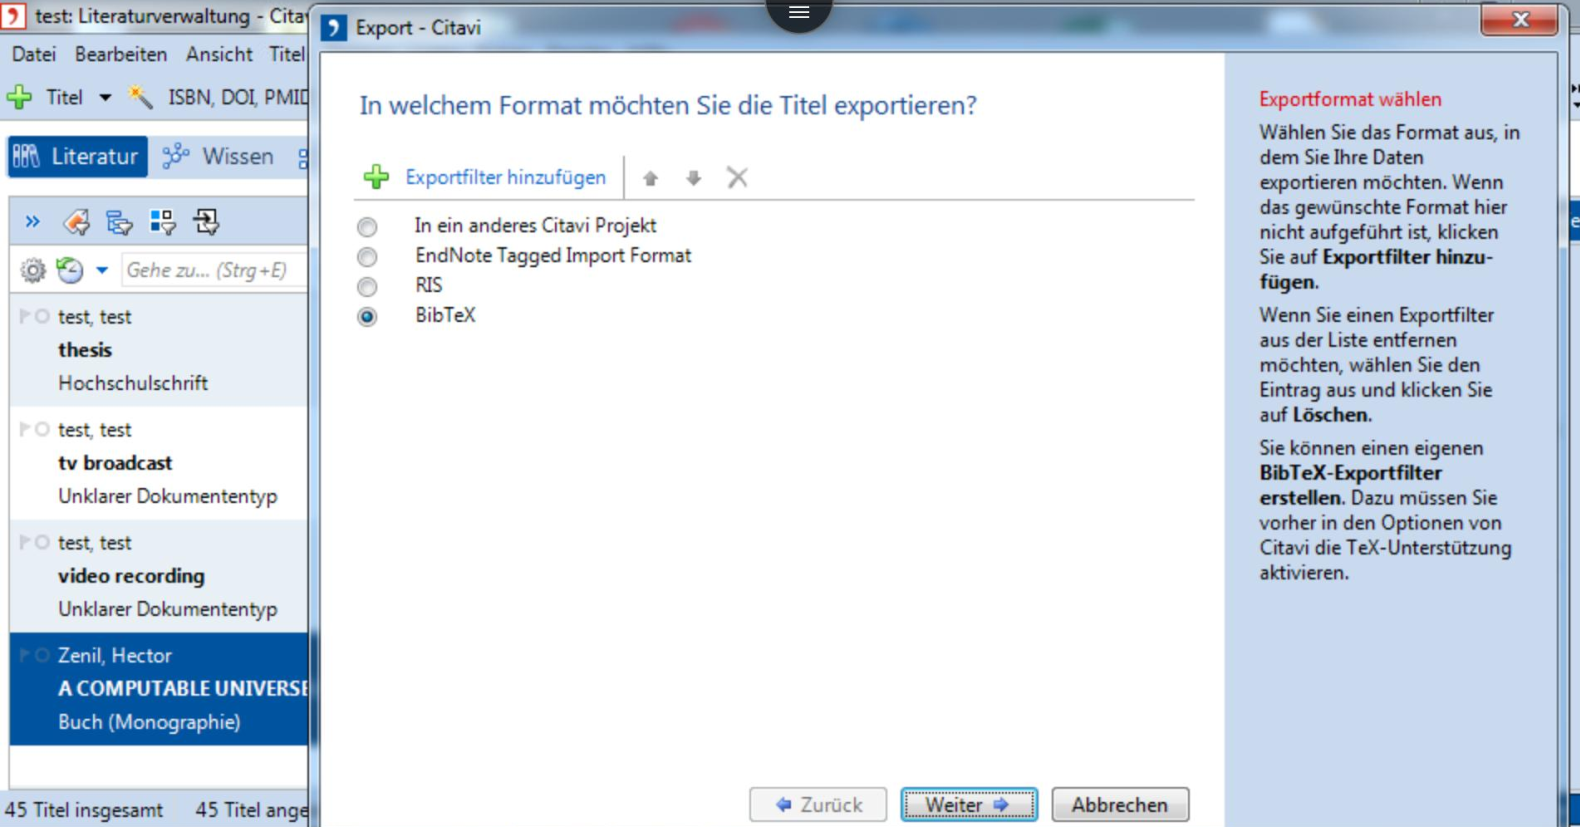
\includegraphics[width=9cm]{Bilder/Kapitel7/Citavi_Schritt3}}
 \caption{Export-Format festlegen}
 \label{fig:exportFormatFestlegen}
\end{figure}
    \item Sie werden nach dem Speicherort gefragt, wählen Sie hier \enquote{Textdaten in der Zwischenablage speichern}. Klicken Sie anschließend auf \enquote{Weiter}.
   
\begin{figure}[h!]
 \centering
 \fbox{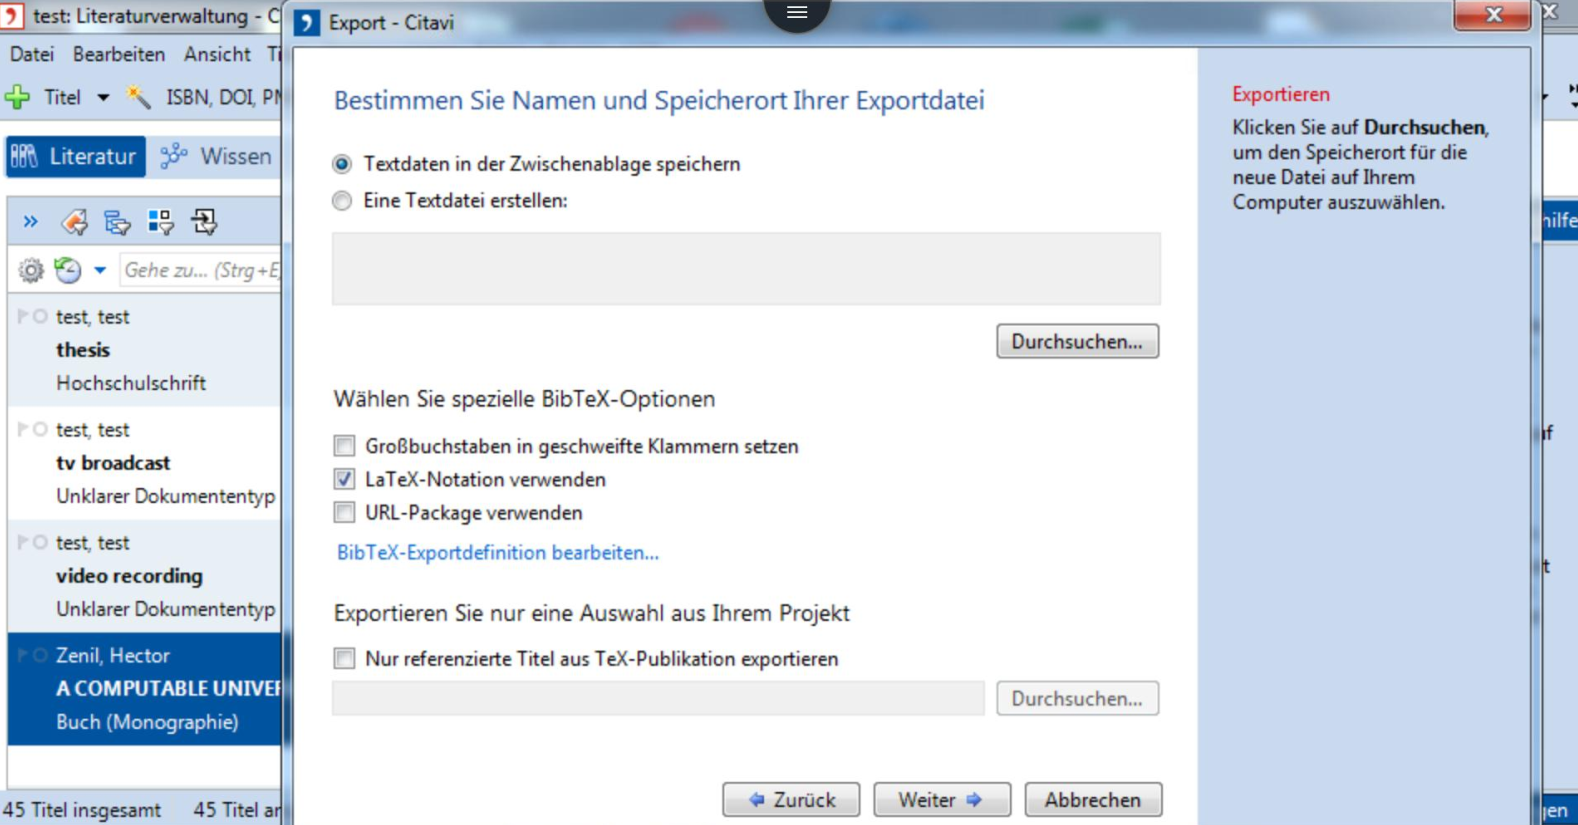
\includegraphics[width=9cm]{Bilder/Kapitel7/Citavi_Schritt4}}
 \caption{Speicherort}
 \label{fig:speicherort}
\end{figure}
    \item Anschließend werden Sie gefragt, ob Sie die Export-Vorlage speichern möchten. Wählen Sie hierfür \enquote{Ja, unter dem Namen:} aus und tragen in das Textfeld \textit{BibTex} als Namen ein. Klicken Sie anschließend auf \enquote{Weiter}.
   
\begin{figure}[h!]
 \centering
 \fbox{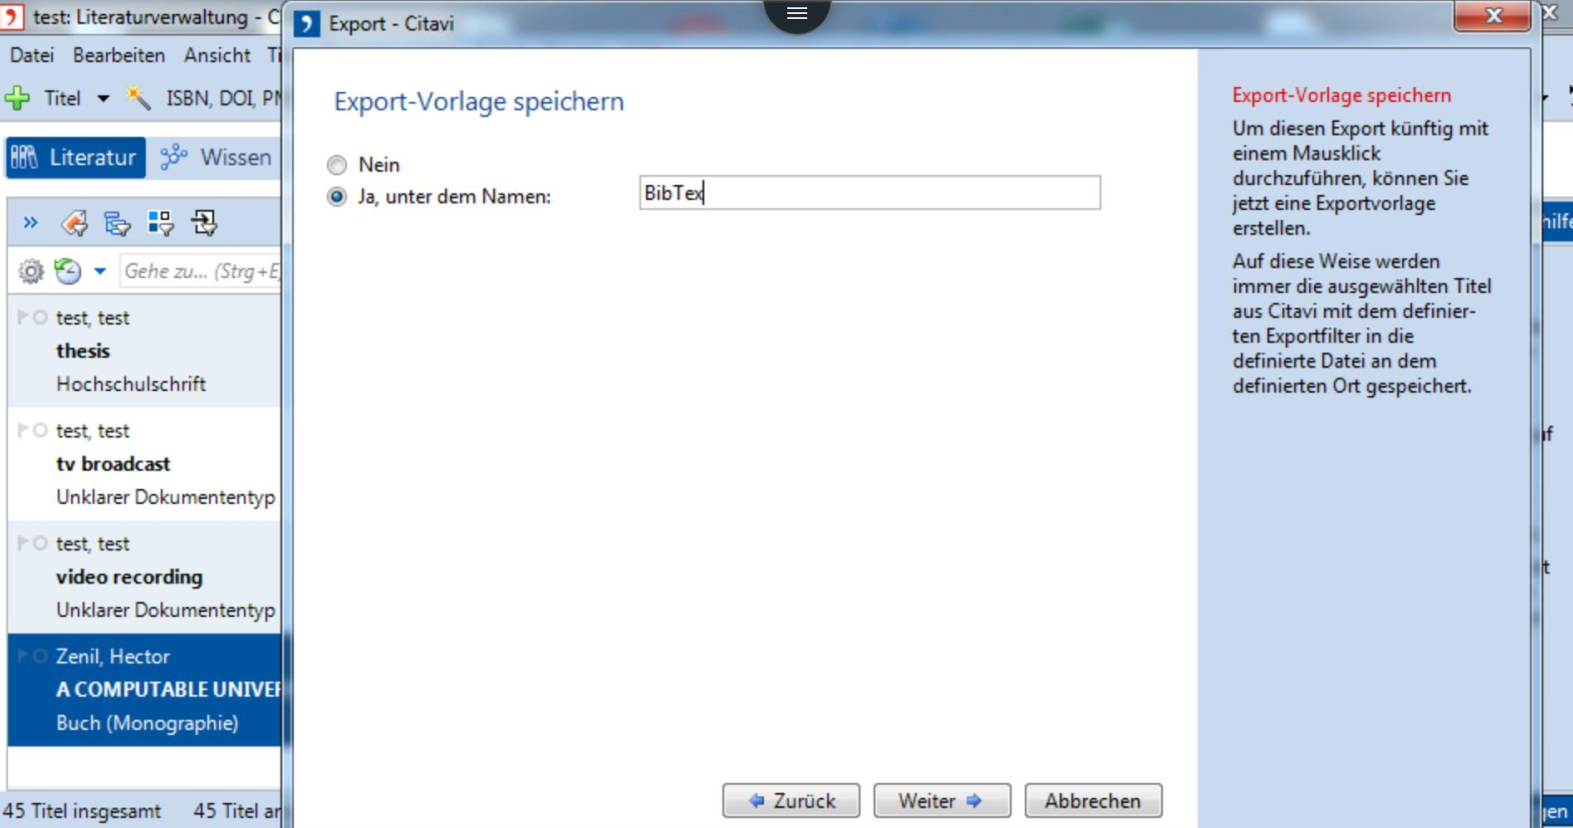
\includegraphics[width=9cm]{Bilder/Kapitel7/Citavi_Schritt5}}
 \caption{Export-Vorlage speichern}
 \label{fig:exportVorlageSpeichern}
\end{figure}
    \item Es öffnet sich ein Popup-Fenster \enquote{Export erfolgreich abgeschlossen}. Bestätigen Sie den Export mit \enquote{OK}.
\end{enumerate}
Die von Ihnen exportierten Daten befinden sich nun in der Zwischenablage. Fahren Sie mit Schritt 1 von BibTex aus der Zwischenablage importieren fort, um Ihre Daten endgültig nach PUMA zu exportieren.\newline

\subsubsection*{Import aus Zotero\index{Import!Zotero}} \label{sss:importZotero}

Um den Import von Zotero\index{Zotero} zu PUMA möglich zu machen, muss Zotero erst einmal für PUMA konfiguriert werden. In den folgenden Schritten erfahren Sie, wie Sie genau vorgehen müssen:
\begin{enumerate}
    \item Öffnen Sie Zotero, indem Sie oben rechts bei Firefox auf das Zotero-Symbol klicken.
    \item Ändern Sie die Einstellungen, indem Sie auf das schwarze Zahnrad klicken. 
\begin{figure}[h!]
 \centering
 \fbox{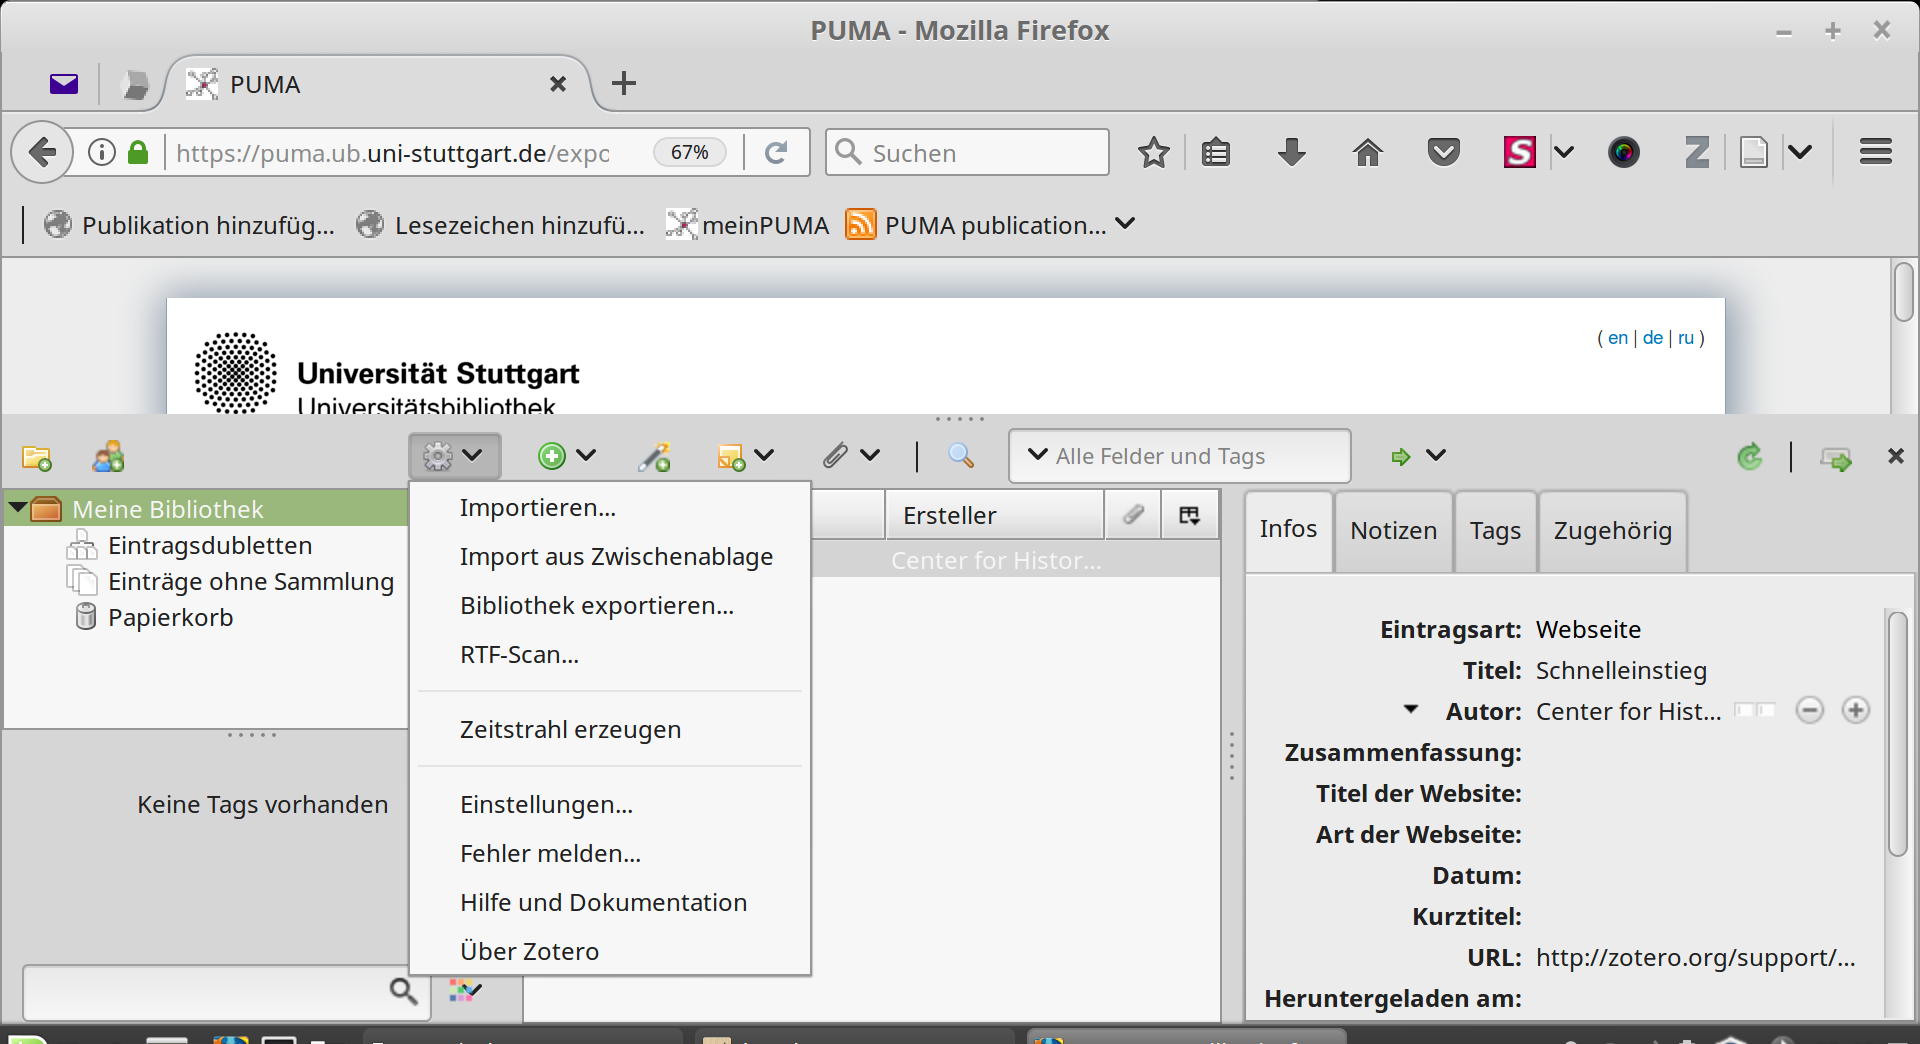
\includegraphics[width=9cm]{Bilder/Kapitel7/Zotero_Import}}
 \caption{Import aus Zotero}
 \label{fig:importZotero}
\end{figure}
    \item Wählen Sie im Dropdown-Menü \enquote{Einstellungen} aus.
    \item Es öffnet sich ein Popup-Fenster, wählen Sie hier den Menüpunkt \enquote{Export} aus.
\begin{figure}[h!]
 \centering
 \fbox{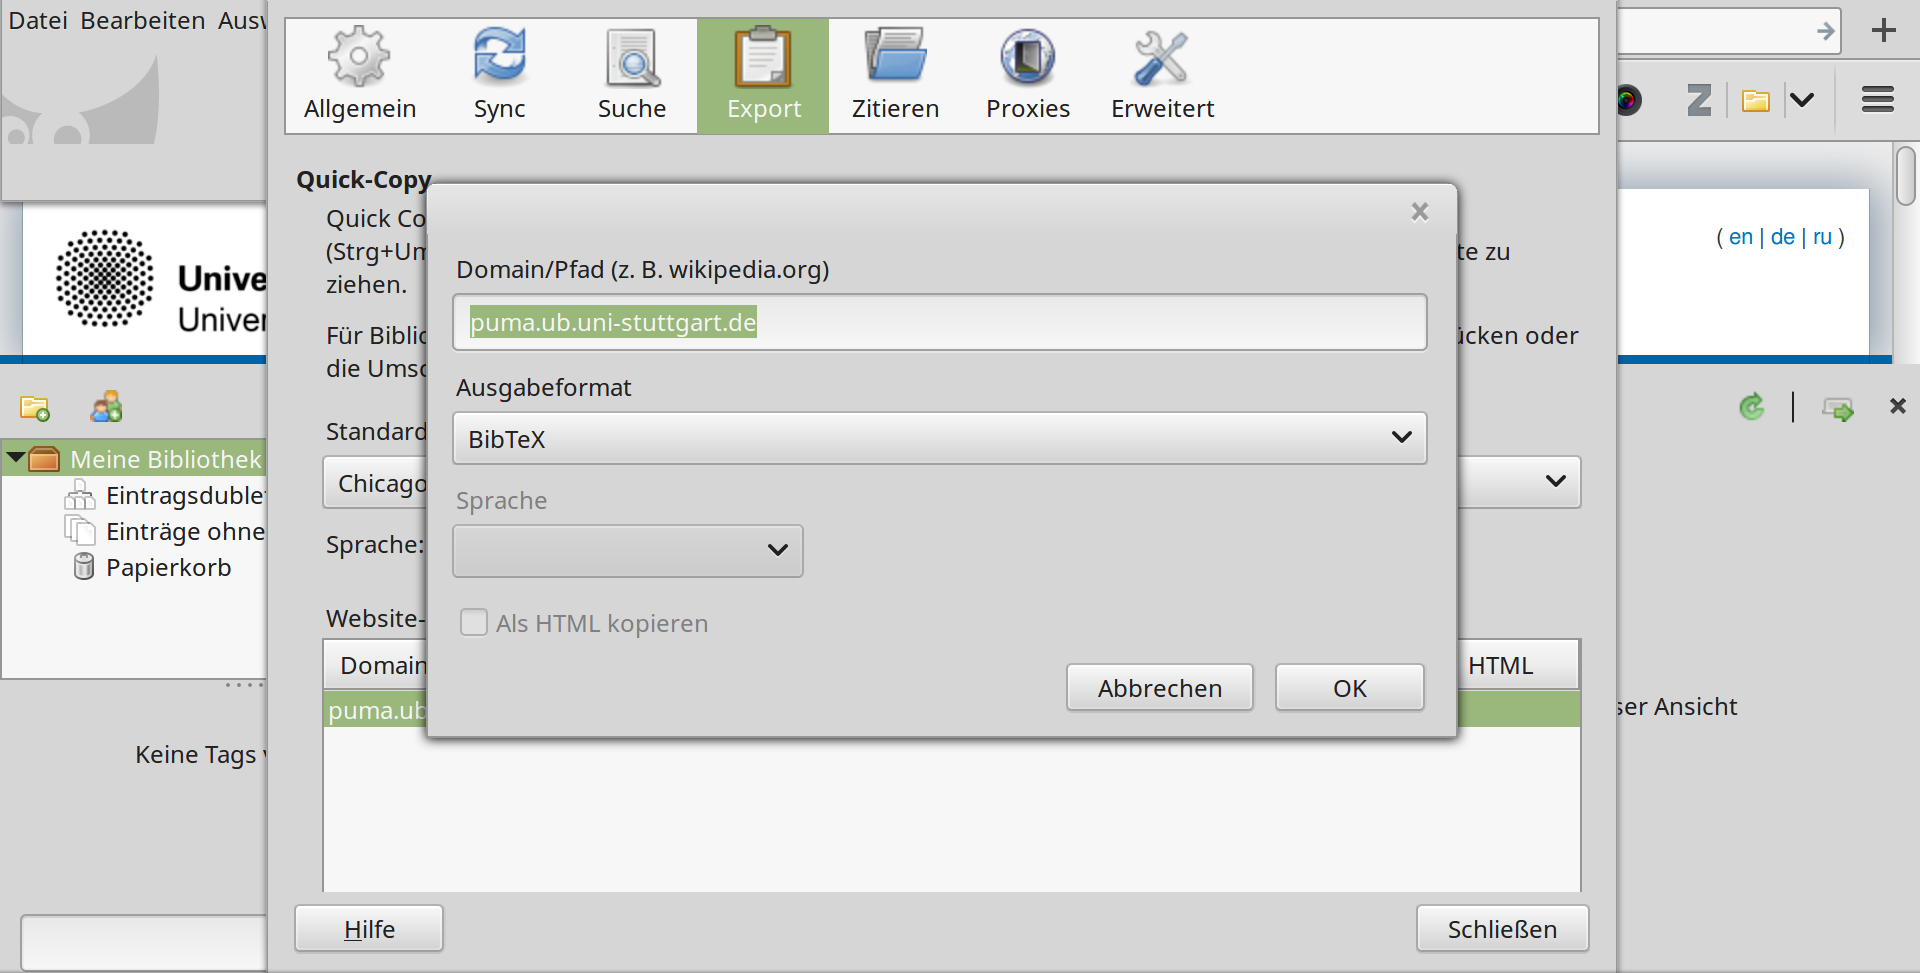
\includegraphics[width=9cm]{Bilder/Kapitel7/Zotero_Menuepunkt_Export}}
 \caption{Menüpunkt Export}
 \label{fig:menueExport}
\end{figure} 
    \item Fügen Sie zu den Website-Spezifischen Einstellungen, durch klicken auf das \enquote{ '+'-Symbol}, einen neuen Eintrag hinzu. Geben Sie in dem Popup-Fenster \textit{puma.ub.uni-stuttgart.de} ein und wählen Sie \textit{BibTeX\index{BibTex}} als Ausgabeformat. Bestätigen Sie den Eintrag mit \enquote{OK}. 
\end{enumerate}
Nachdem Sie die Konfiguration vorgenommen haben, können Sie die Publikationen nach PUMA importieren. 
\begin{enumerate}
    \item Klicken Sie im Hauptmenü auf \enquote{Eintragen} und wählen im Dropdown-Menü die Option \enquote{Publikation eintragen} aus.  
    \item Klicken Sie auf den Reiter \enquote{BibTex\index{BibTex}/EndNote\index{EndNote}-Schnipsel}. In das Feld \enquote{Auswahl} können Sie nun den entsprechenden Eintrag aus Ihrer Zotero-Bibliothek durch Drag und Drop hineinziehen (klicken Sie auf den Zotero-Eintrag, halten Sie die linke Maustaste gedrückt, bewegen Sie den Mauszeiger in das Feld und lassen Sie dann die linke Maustaste los). Durch Klicken auf \enquote{Weiter} werden die Daten aus dem Zotero-Eintrag extrahiert und in die entsprechenden Felder eingetragen. 
\begin{figure}[h!]
 \centering
 \fbox{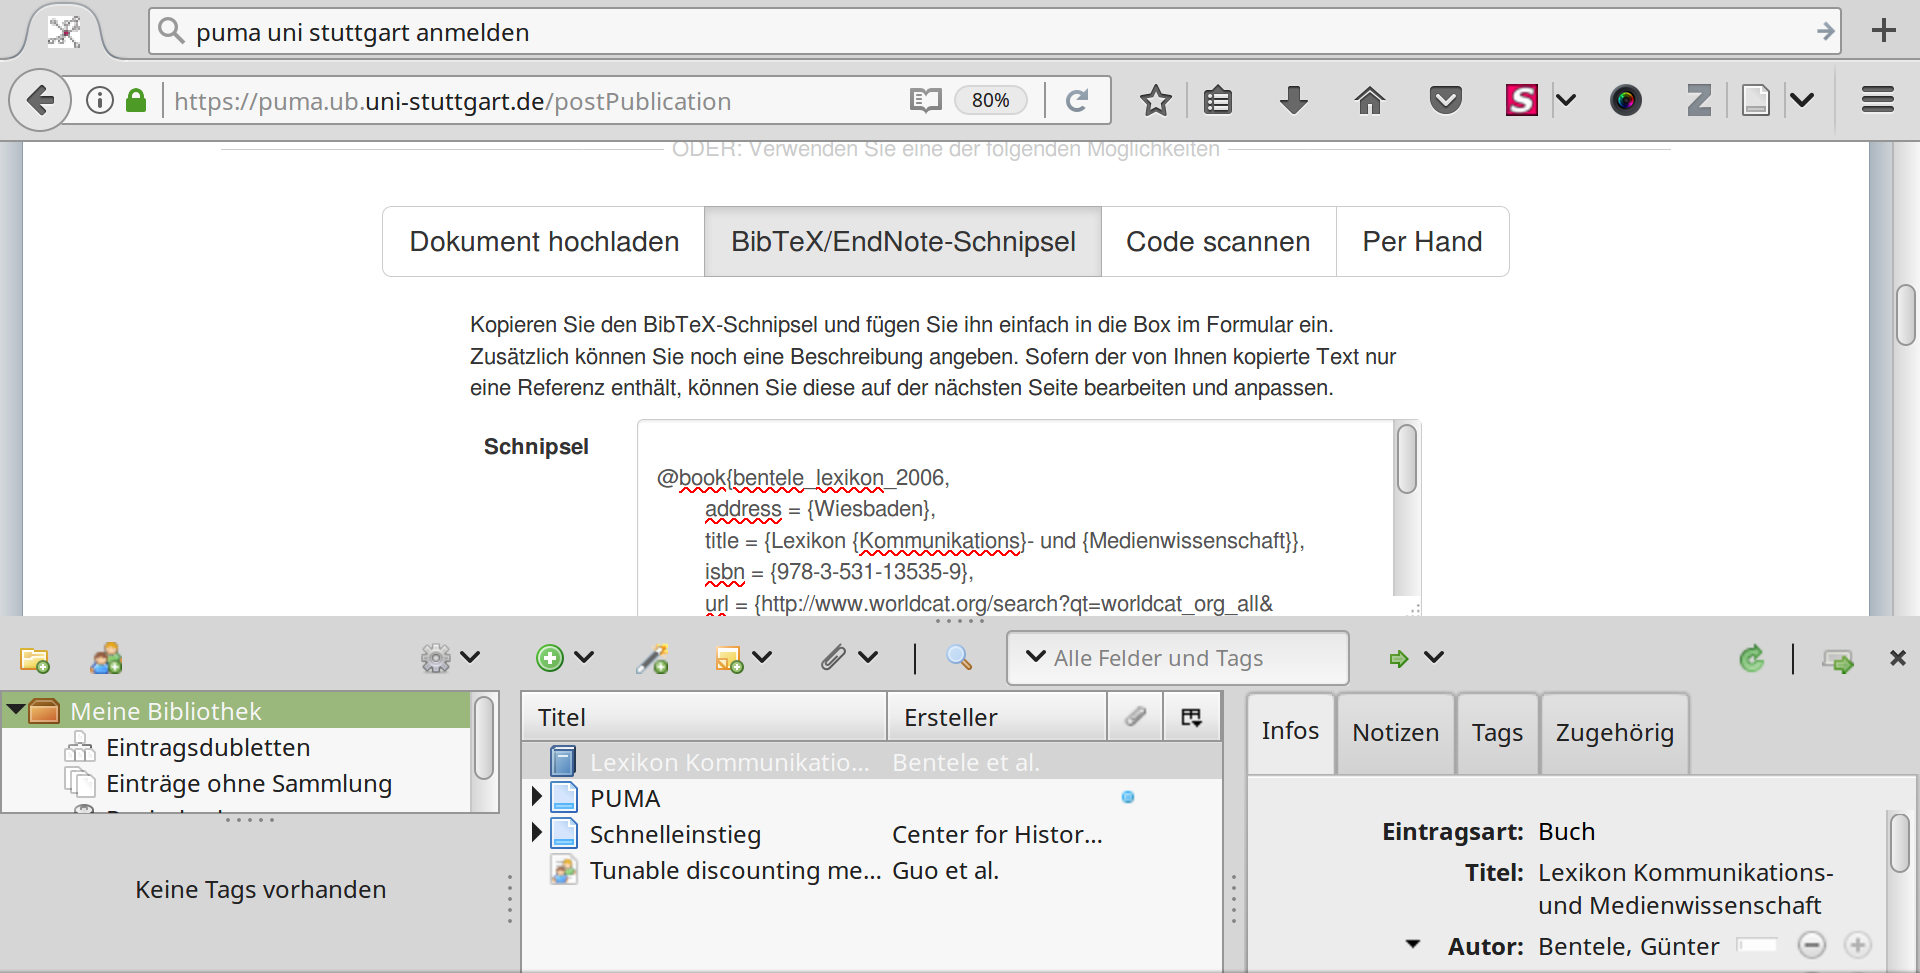
\includegraphics[width=10cm]{Bilder/Kapitel7/Zu_PUMA_importieren}}
 \caption{Zu PUMA importieren}
 \label{fig:zuPumaImportieren}
\end{figure}
    \item Klicken Sie anschließend auf \enquote{Speichern} um den Eintrag in Ihre Sammlung zu übernehmen.
\end{enumerate}  
\subsubsection{Import aus JabRef\index{Import!JabRef}\index{JabRef}}\label{sss:importJabRef}
\begin{enumerate}
    \item Klicken Sie mit der rechten Maustaste auf die Publikation, die Sie nach PUMA importieren möchten.
    \item Es erscheint ein Dialog. Wählen Sie \enquote{In die Zwischenablage kopieren} aus.
    \item Im nächsten Schritt werden Sie nach dem Export-Format gefragt, wählen Sie hier \enquote{Endnote} aus.
\end{enumerate}
Die von Ihnen exportierte Publikation befindet sich nun in der Zwischenablage. Fahren Sie mit Schritt 1 von BibTex/~EndNote aus der Zwischenablage importieren fort, um Ihre Publikation endgültig nach PUMA zu exportieren.

\subsection{BibTex\index{BibTex}/ EndNote\index{EndNote} aus der Zwischenablage importieren}
\label{subsec:bibtexImportieren}
Voraussetzung ist, dass Sie Ihre Literaturliste aus Ihrem bisherigen Literaturverwaltungsprogramm in die Zwischenablage exportieren.
\begin{enumerate}
    \item Klicken Sie auf den Menüpunkt \enquote{Eintragen} im Hauptmenü. Ein Untermenü klappt auf.
    \item Klicken Sie im Untermenü auf \enquote{Publikation eintragen}.
    \item Klicken Sie auf den Reiter \enquote{BibTex/~EndNote-Schnipsel}.
    \item Fügen Sie den Text aus der Zwischenablage in das Textfeld \enquote{Auswahl} ein. Dies können Sie so erreichen, indem Sie auf das Textfeld Auswahl gehen und mit der rechte Maustaste das Menü öffnen und auf \enquote{Einfügen} klicken. Erscheint das \enquote{Einfügen} grau, dann haben Sie keine Daten in die Zwischenablage exportiert und Sie müssen den Text erneut in die Zwischenablage einfügen.
    \item Klicken Sie auf \enquote{Weiter}.
    \item PUMA zeigt Ihnen nun eine Übersicht über alle Daten an. Überprüfen Sie diese auf ihre Richtigkeit.
    \item Klicken Sie \enquote{Speichern}.
\end{enumerate}
\section{RSS-Feed abonnieren} 
\label{sec:rssFeedAbonnieren}
RSS\index{RSS} (engl. Really Simple Syndication)-Feeds sind Dateienformate, die Ihnen Veränderungen auf Websites zeigen. So werden Sie immer über Neuigkeiten informiert. Für PUMA bedeutet der RSS-Feed, dass Sie eigene oder fremde Publikations-/~Lesezeichenlisten abonnieren können. Dies funktioniert auch mit Publikationslisten von Gruppen. Nach dem Abonnieren werden Sie über jede Neuigkeit (z.~B. Neue Einträge) informiert. 
\begin{enumerate}
    \item Klicken Sie auf das Exportzeichen in der Publikations-/~Lesezeichenspalte, die Sie abonnieren wollen. Es öffnet sich ein Dropdown- Menü.
\begin{figure}[h!]
 \centering
 \fbox{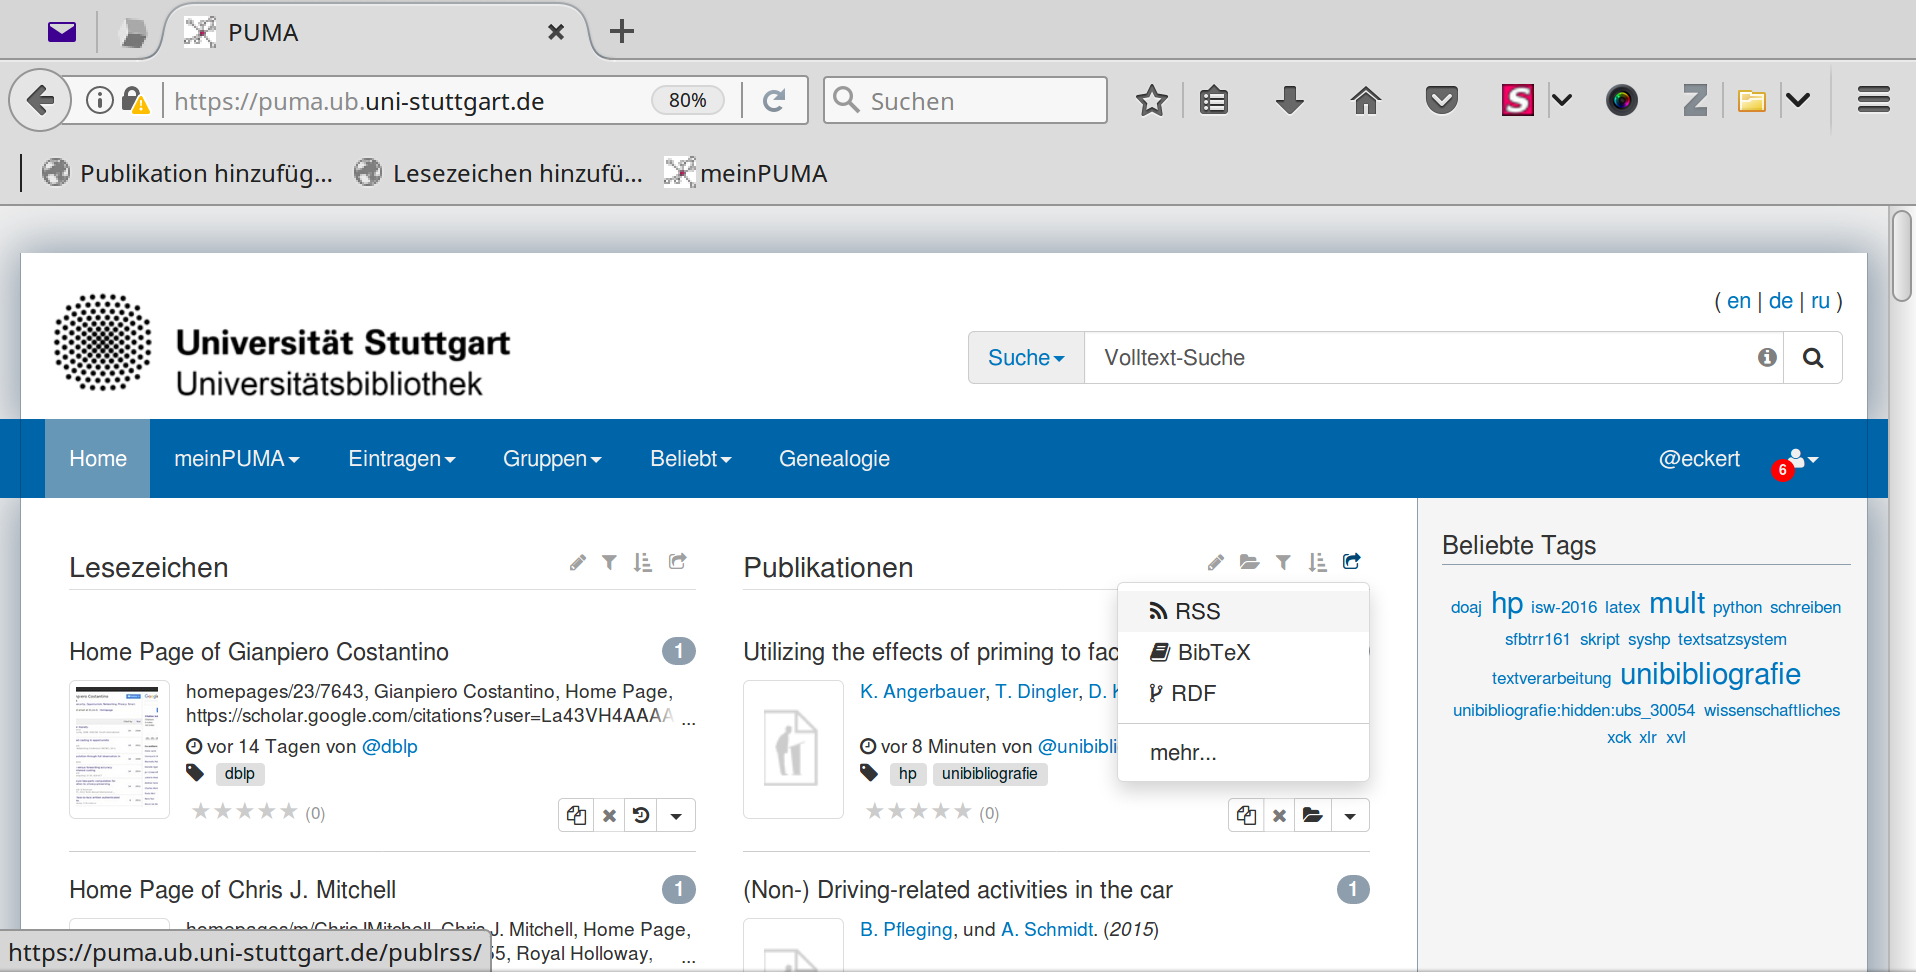
\includegraphics[width=10cm]{Bilder/Kapitel7/RSS-feed_abonnieren}}
 \caption{RSS-Feed abonnieren}
 \label{fig:rssFeedAbbonnieren}
\end{figure}
    \item  Klicken Sie auf \enquote{RSS}. Der RSS-Feed wird erzeugt und an Ihren RSS-Reader weitergeleitet. 
\begin{mdframed}[style=mdfexample1,frametitle={\texttt{ACHTUNG}},backgroundcolor=gray!40]\texttt{Das weitere Vorgehen ist exemplarisch, es richtet sich sowohl nach Ihrem Webbrowser als auch nach Ihrem RSS-Reader. Im gezeigten Fall übernimmt der Browser \enquote{Mozilla Firefox} sowohl die Aufgabe des Webbrowsers als auch die des RSS-Readers.}
\end{mdframed}
    \item Es werden Ihnen von Mozilla Firefox einige Optionen zum Abonnieren angeboten. Wählen Sie hier \enquote{Dynamische Lesezeichen} und klicken Sie anschließend auf \enquote{Jetzt abonnieren}.
\begin{figure}[h!]
 \centering
 \fbox{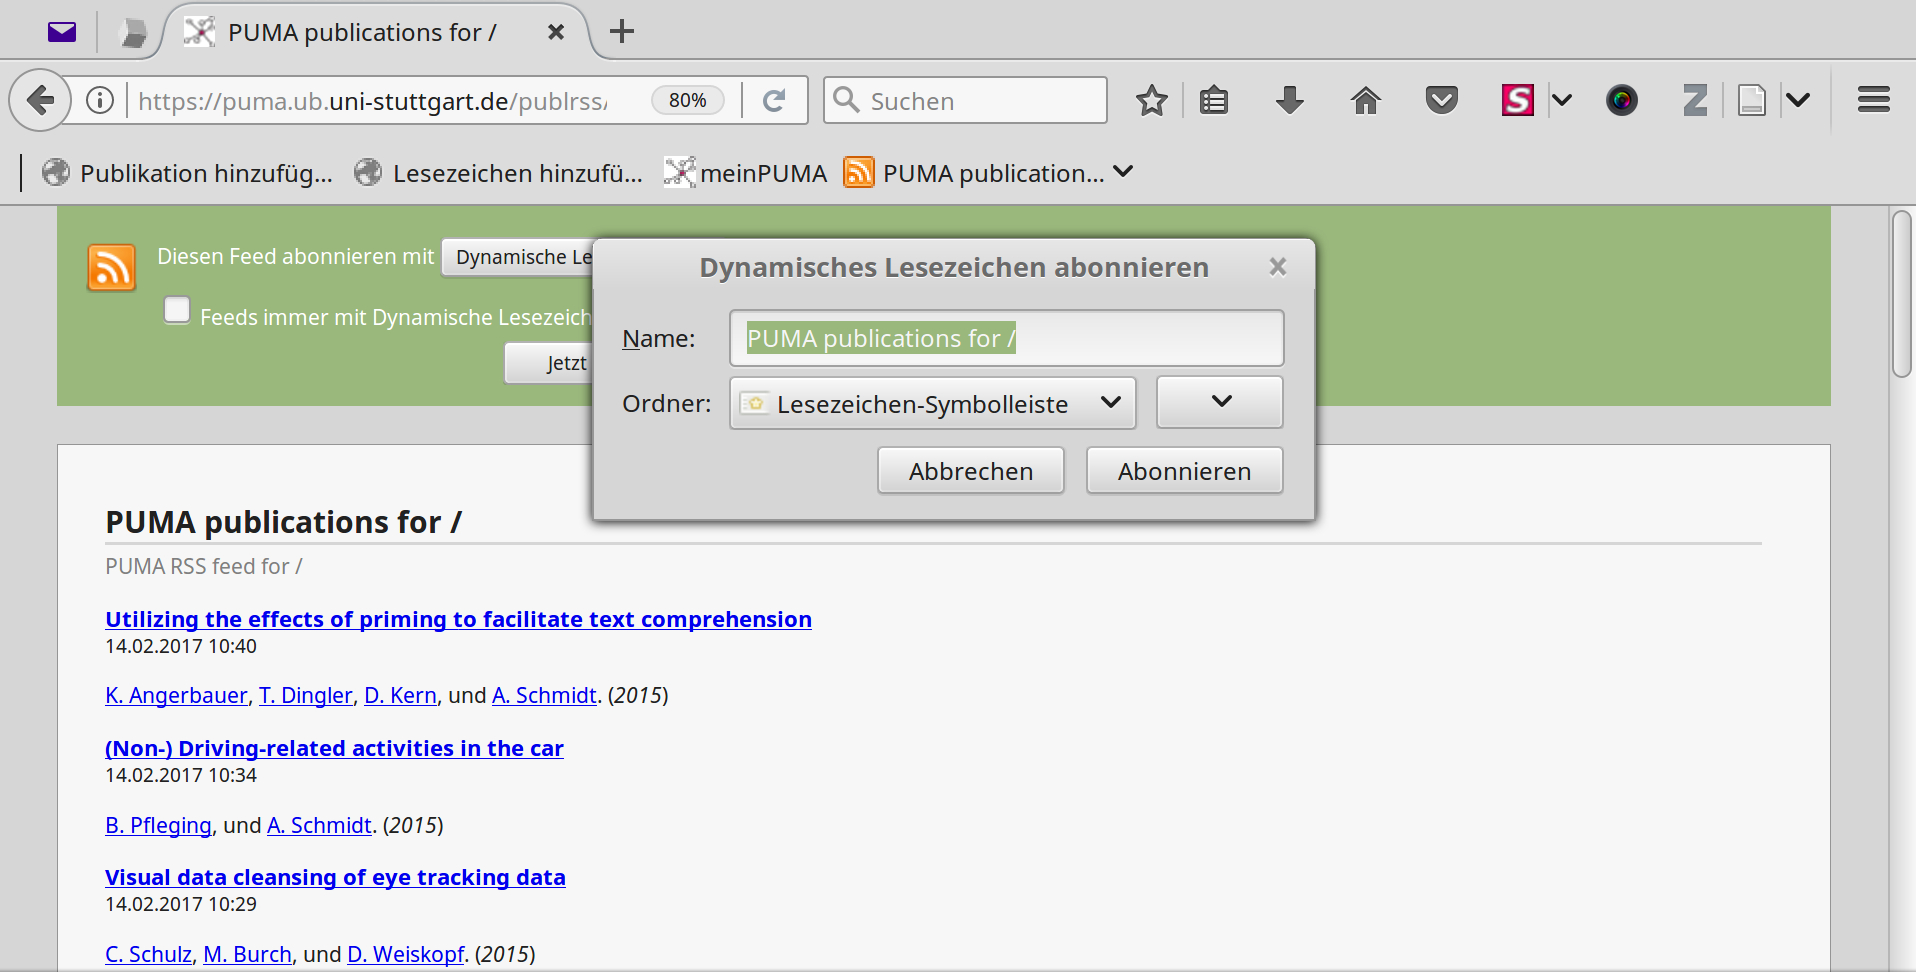
\includegraphics[width=11cm]{Bilder/Kapitel7/RSS_dynamisches_Lesezeichen}}
 \caption{Das dynamische Lesezeichen}
 \label{fig:dynamischesLesezeichen}
\end{figure}
    \item Ein Pop-Up Fenster öffnet sich. Wählen Sie einen Namen für den RSS-Feed aus. PUMA generiert immer automatisch einen Namen, diesen können Sie übernehmen.
    \item Wählen Sie den Ordner aus, in dem der RSS-Feed gespeichert werden soll.
    \item Klicken Sie abschließend auf \enquote{Abonnieren}, um den Feed zu abonnieren/speichern.
\end{enumerate}
Dies ist nun die Ansicht des RSS-Feeds-Readers im Vergleich zur Ansicht in PUMA:
\begin{figure}[h!]
 \centering
 \fbox{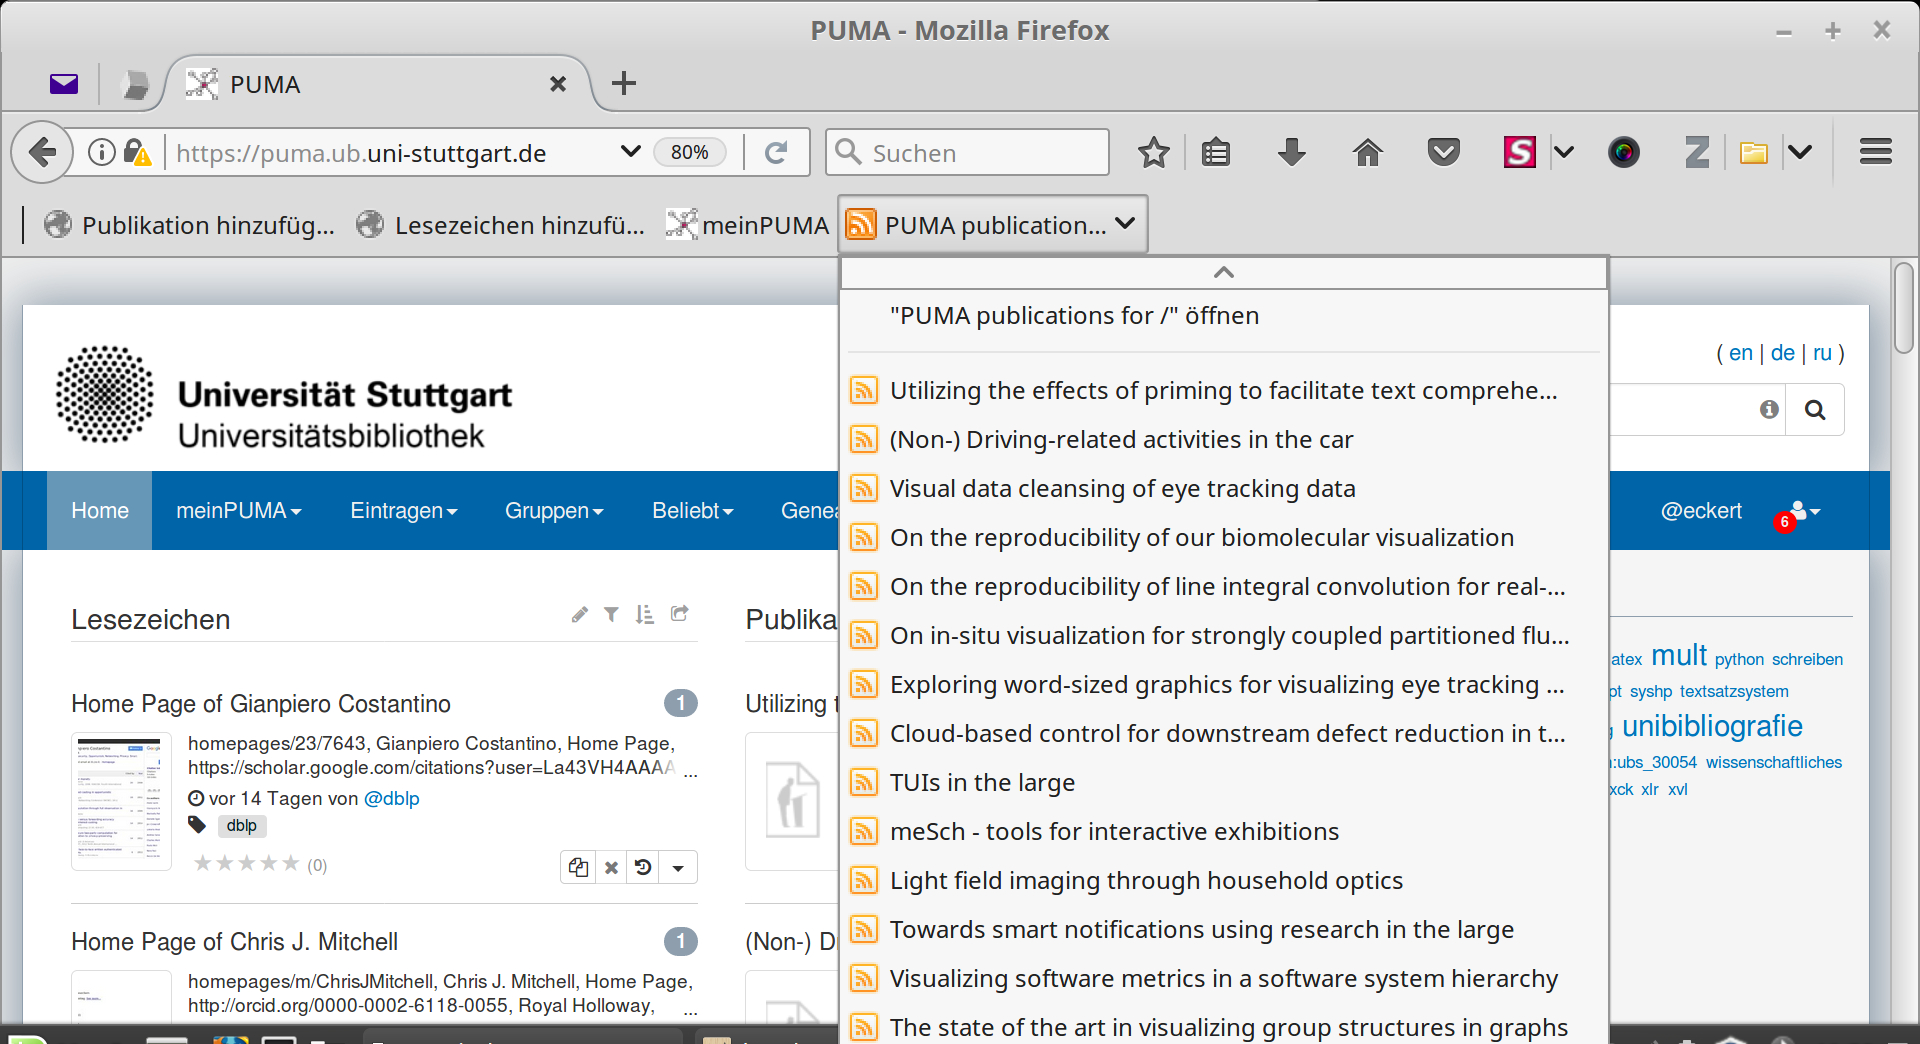
\includegraphics[width=11cm]{Bilder/Kapitel7/RSS-Reader}}
 \caption{Der RSS-Reader}
 \label{fig:rssReader}
\end{figure}
\section{Universitätsbibliografie\index{Unibibliografie}}
\label{sec:unibibliografie}
Die Universitätsbibliografie (kurz: Unibibliografie) bietet eine möglichst vollständige Übersicht über die Publikationen, die an der Universität Stuttgart veröffentlicht werden. Seit 2015 werden sämtliche Publikationen aller wissenschaftlichen Mitglieder (nach §9 LHG) der Universität Stuttgart hier gezeigt, die während und ggf. nach ihrer Zugehörigkeit zur Universität verfasst bzw. herausgegeben, öffentlich und dauerhaft verfügbar gemacht wurden.\newline\newline
Geführt wird die Unibibliografie der Universität Stuttgart über PUMA. Für die Mitglieder der Universität besteht zukünftig auch die Möglichkeit ihre Publikationen über PUMA zu melden. Die Universitätsbibliothek bearbeitet die Datensätze und veröffentlicht diese Publikationsmetadaten in der Gruppe \textit{unibibliografie} in PUMA. Das System bietet sehr viele Möglichkeiten, die gewünschten Daten zu exportieren. Weitere Informationen finden Sie auf der Homepage der Universitätsbibliothek Stuttgart. \footnote{\url{http://www.ub.uni-stuttgart.de/forschen-publizieren/unibibliografie/}}
\section{OPUS}
\label{sec:opus}
\subsection{Über OPUS}
\label{subsec:ueberOpus}
OPUS ist der Dokumentenserver (das institutionelle Repositorium) der Universität Stuttgart. Die Möglichkeit, über OPUS zu veröffentlichen ist, ist derzeit noch in der Planung. Alle Angehörigen der Universität Stuttgart können in der Zukunft über OPUS ihre Dokumente, die von dauerhaftem Interesse für Forschung und Lehre sind, online im Sinne von Open Access\index{Open Access} veröffentlichen.
\newline\newline
Es wird die Möglichkeit bestehen, dass die Nutzer von PUMA aus in OPUS\index{OPUS} veröffentlichen können. Bei der Aktivierung des Tags \textit{myown}, wird den Nutzern automatisch die Veröffentlichung auf OPUS angeboten werden. Durch diesen Schritt werden ihre Publikationen im Internet langfristig und weltweit frei zugänglich. Dadurch werden die Veröffentlichungen auch in Bibliothekskatalogen, Datenbanken und allen gängigen Suchmaschinen nachgewiesen und somit die Sichtbarkeit der Publikationen deutlich erhöht.
\newline\newline
Die Zitierfähigkeit der Veröffentlichungen wird durch eine dauerhafte, stabile Internet-Adresse (Persistent Identifier) garantiert.
\newline\newline
Mit dem Repositorium wird der von der Universität Stuttgart geförderte freie Zugang zu wissenschaftlicher Information (Open Access) unterstützt werden.
%\subsection{OPUS und PUMA}
%\label{subsec:opusPuma}
%Beim Eintragen einer Veröffentlichung/Publikation in PUMA wird die eigene Veröffentlichung mit \textit{myown} getaggt. Sie werden von PUMA gefragt, ob Sie auf OPUS veröffentlichen wollen. Wenn Sie diese Frage mit \enquote{Ja} bestätigen, wird eine SWORD-Datenverbindung\index{SWORD} zur Sherpa/Romeo-Liste\index{Sherpa/Romeo-Liste} hergestellt. Diese zeigt an, was die Verlage im Bezug auf die Veröffentlichung erlauben. Ist das Hochladen \enquote{grün}, so wird die Veröffentlichung auf OPUS  hochgeladen (so genanntes \enquote{Self Archiving}).
%\newline \newline
%Die Sherpa/Romeo-Liste\footnote{\url{http://www.sherpa.ac.uk/romeo/index.php}} ist eine Datenbank in Manchester, über die die Verlagskonditionen für Zweitveröffentlichungen abgefragt werden können. Bei deutschen Verlagen gilt ein Zeitfenster von 12 Monate nach Erstveröffentlichung, bevor die Autoren eine Zweitveröffentlichung machen können (Grüner Weg des Open Access). Bei Verlagen im Ausland gelten z. T. deutlich höhere Schutzfristen.
\section{DBLP}
\label{dblp}
Das Digital Bibliography \& Library Project (DBLP\index{DBLP}; zu deutsch: Digitales Bibliographie- und Bibliotheksprojekt) ist eine online verfügbare bibliographische Datenbank. In der Sammlung befinden sich mehr als 3 Mio. unterschiedliche wissenschaftliche Publikationen aus dem Bereich Informatik.\newline
PUMA und BibSonomy sind mit der DBLP-Datenbank verbunden. Die Datenbank wird mehrmals wöchentlich aktualisiert und stellt PUMA und BibSonomy Publikationen zur Nachnutzung zur Verfügung. \newline
Die Nutzer können so, die in PUMA hochgeladenen Publikationen und Lesezeichen nachnutzen und mit ein paar Klicks in die eigenen Sammlung übernehmen. 
